% !TEX program = xelatex
\documentclass[11pt,a4paper,fontset=windows]{ctexart}

\usepackage[top=2.3cm,bottom=2.3cm,left=2.3cm,right=2.3cm,headheight=22pt]{geometry}
\usepackage{graphicx}
\usepackage{xcolor}
\usepackage{booktabs}
\usepackage{tabularx}
\usepackage{array}
\usepackage{longtable}
\usepackage{enumitem}
\usepackage{caption}
\usepackage{float}
\usepackage{titlesec}
\usepackage{fancyhdr}
\usepackage[most]{tcolorbox}
\usepackage{listings}
\usepackage{tikz}
\usetikzlibrary{positioning,arrows.meta,calc,shapes.geometric,fit,backgrounds}
\usepackage{pgfplots}
\pgfplotsset{compat=1.18}
\usepackage{amsmath}
\usepackage{etoolbox}
\AtBeginEnvironment{longtable}{\footnotesize}
\usepackage[hidelinks,unicode]{hyperref}

\definecolor{ink}{HTML}{1F4D3A}
\definecolor{inklight}{HTML}{3C6E57}
\definecolor{sand}{HTML}{F3EEE3}
\definecolor{line}{HTML}{D8D0C0}
\definecolor{muted}{HTML}{6B6459}
\definecolor{palegreen}{HTML}{E8F0EA}
\definecolor{warn}{HTML}{A34A32}
\definecolor{amber}{HTML}{B8842F}

\captionsetup{font=small,labelfont=bf,labelsep=quad,skip=5pt}
\renewcommand{\figurename}{图}
\renewcommand{\tablename}{表}
\renewcommand{\lstlistingname}{代码清单}
\renewcommand{\arraystretch}{1.14}
\setlength{\tabcolsep}{4.5pt}
\newcolumntype{L}[1]{>{\raggedright\arraybackslash}p{#1}}
\newcolumntype{C}[1]{>{\centering\arraybackslash}p{#1}}
\newcolumntype{Y}{>{\raggedright\arraybackslash}X}

\titleformat{\section}{\Large\bfseries\color{ink}}{\thesection}{0.8em}{}
\titleformat{\subsection}{\large\bfseries\color{inklight}}{\thesubsection}{0.7em}{}
\titleformat{\subsubsection}{\normalsize\bfseries\color{inklight}}{\thesubsubsection}{0.6em}{}
\titlespacing*{\section}{0pt}{15pt}{7pt}
\titlespacing*{\subsection}{0pt}{11pt}{5pt}
\titlespacing*{\subsubsection}{0pt}{8pt}{3pt}

\pagestyle{fancy}
\fancyhf{}
\fancyhead[L]{\small\color{muted}一纸成课（Paper2Lesson）· 作品介绍}
\fancyhead[R]{\small\color{muted}v0.1.6}
\fancyfoot[C]{\small\thepage}
\renewcommand{\headrulewidth}{0.4pt}
\renewcommand{\headrule}{\hbox to\headwidth{\color{line}\leaders\hrule height \headrulewidth\hfill}}

\setlength{\parskip}{0.28em}
\setlength{\parindent}{2em}
\linespread{1.30}
\setlist[itemize]{leftmargin=2em,itemsep=2.5pt,topsep=3pt}
\setlist[enumerate]{leftmargin=2.2em,itemsep=2.5pt,topsep=3pt}
\setlength{\emergencystretch}{2em}

\newcommand{\env}[1]{\texttt{\detokenize{#1}}}
\newcommand{\file}[1]{\nolinkurl{#1}}
\newcommand{\good}[1]{\textcolor{ink}{\textbf{#1}}}
\newcommand{\repo}{\url{https://github.com/Td12138/yizhi-chengke}}

\lstset{
  basicstyle=\ttfamily\small,
  breaklines=true,
  breakatwhitespace=false,
  columns=fullflexible,
  frame=single,
  rulecolor=\color{line},
  backgroundcolor=\color{sand},
  keywordstyle=\color{ink}\bfseries,
  commentstyle=\color{muted},
  stringstyle=\color{inklight},
  showstringspaces=false,
  xleftmargin=0.7em,
  xrightmargin=0.7em,
  aboveskip=0.8em,
  belowskip=0.8em,
  captionpos=b,
  extendedchars=false
}
\lstdefinelanguage{json}{
  basicstyle=\ttfamily\small,
  showstringspaces=false,
  breaklines=true,
  morestring=[b]",
  literate=*{0}{{{\color{inklight}0}}}{1}{1}{{{\color{inklight}1}}}{1}
    {2}{{{\color{inklight}2}}}{1}{3}{{{\color{inklight}3}}}{1}
    {4}{{{\color{inklight}4}}}{1}{5}{{{\color{inklight}5}}}{1}
    {6}{{{\color{inklight}6}}}{1}{7}{{{\color{inklight}7}}}{1}
    {8}{{{\color{inklight}8}}}{1}{9}{{{\color{inklight}9}}}{1}
}

\newtcolorbox{keybox}[1][]{
  enhanced,breakable,colback=sand,colframe=line,boxrule=0.5pt,arc=2pt,
  left=8pt,right=8pt,top=6pt,bottom=6pt,
  fonttitle=\bfseries\color{ink},title=#1
}
\newtcolorbox{warnbox}[1][]{
  enhanced,breakable,colback=warn!5,colframe=warn!45,boxrule=0.5pt,arc=2pt,
  left=8pt,right=8pt,top=6pt,bottom=6pt,
  fonttitle=\bfseries\color{warn},title=#1
}

\begin{document}

% 封面
\begin{titlepage}
\thispagestyle{empty}
\begin{tikzpicture}[remember picture,overlay]
  \fill[ink] (current page.north west) rectangle ([yshift=-10.5cm]current page.north east);
  \fill[sand] ([yshift=-10.5cm]current page.north west) rectangle ([yshift=-10.72cm]current page.north east);
  \node[anchor=north west,text=white,align=left] at ([xshift=2.0cm,yshift=-1.45cm]current page.north west) {
    {\small 全国大学生计算机应用能力与数字素养大赛}\\[3pt]
    {\small 暨第九届传智杯全国大学生数智创新与 AI 应用大赛}
  };
  \node[anchor=north west,text=white,align=left] at ([xshift=2.0cm,yshift=-3.05cm]current page.north west) {
    {\fontsize{48}{54}\selectfont\bfseries 一纸成课}\\[7pt]
    {\fontsize{22}{28}\selectfont Paper2Lesson}
  };
  \node[anchor=north west,text=white!92,align=left] at ([xshift=2.0cm,yshift=-6.65cm]current page.north west) {
    {\Large 作品介绍文档}\\[9pt]
    {\large 拍下一页纸，生成可追问、可练习、可讲解、可批改的课程}\\[7pt]
    {\normalsize 符号验算 · 分步诊断 · 带出处的检索 · 七 Agent 可观测编排}
  };
  \node[anchor=north east,text=white,align=right] at ([xshift=-2.0cm,yshift=-8.95cm]current page.north west) {
    {\small AI 创新应用挑战赛（个人赛 / 技术应用赛）}
  };
\end{tikzpicture}

\vspace*{10.15cm}
\begin{center}
  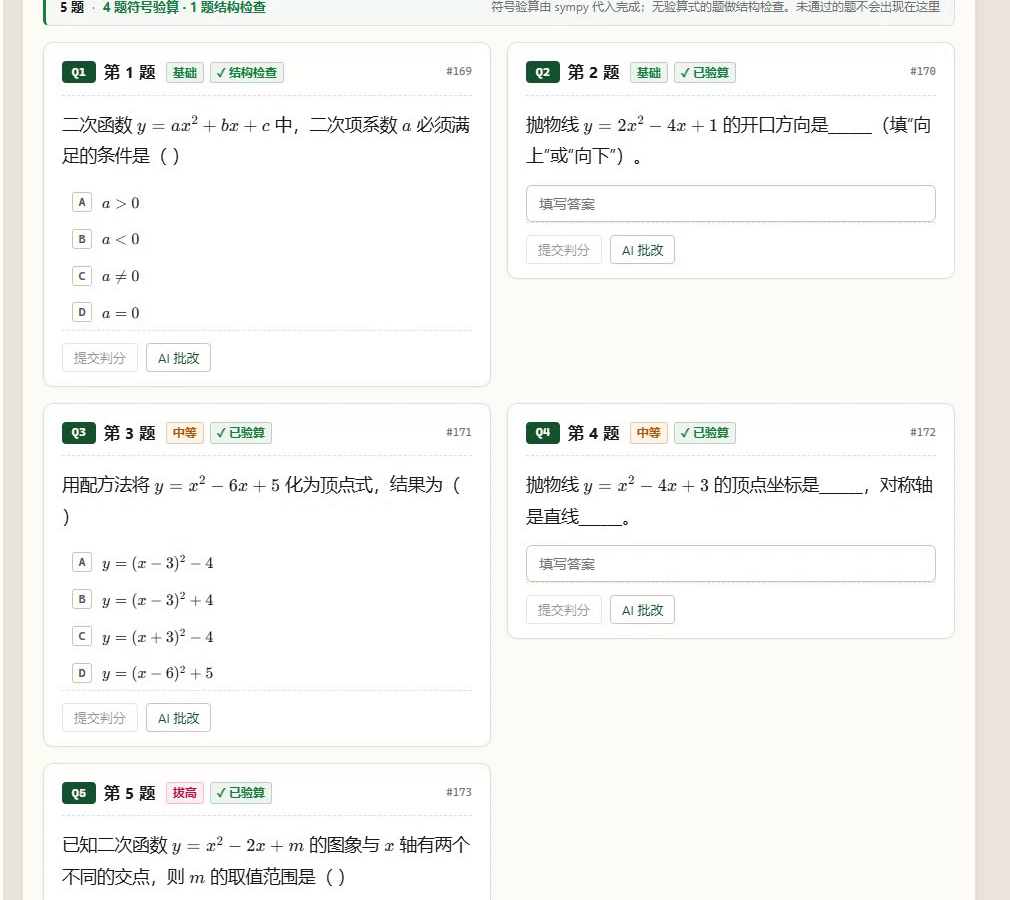
\includegraphics[width=0.72\textwidth,height=7.0cm,keepaspectratio]{img/c03.png}
\end{center}
\vfill
\begin{center}
\small
\begin{tabularx}{0.94\textwidth}{@{}>{\bfseries\color{ink}}L{2.3cm}Y@{}}
\toprule
作品版本 & v0.1.6 \\
作品形态 & Windows 免安装桌面版、单文件便携版、Web 源码 \\
代码仓库 & \repo \\
开源许可 & 源码 MIT；桌面二进制含 AGPL 组件，许可义务见附录 D \\
文档日期 & 2026 年 11 月 18 日 \\
\bottomrule
\end{tabularx}
\end{center}
\end{titlepage}

% 文档信息表
\pagenumbering{Roman}
\section*{文档信息}
\addcontentsline{toc}{section}{文档信息}
\begin{table}[H]
\centering
\footnotesize
\caption{作品介绍文档信息表}
\begin{tabularx}{0.96\textwidth}{@{}L{3.0cm}Y@{}}
\toprule
\textbf{项目} & \textbf{内容} \\
\midrule
作品名称 & 一纸成课（Paper2Lesson） \\
参赛赛道 & AI 创新应用挑战赛，个人赛 / 技术应用赛 \\
核心定位 & 将纸面资料转为知识卡片，再完成命题、验算、练习、批改、讲解与检索 \\
当前版本 & v0.1.6；本文数字均对应该版本，历史版本数据单独注明 \\
代码仓库 & \repo \\
交付形态 & Web 源码、Windows 目录版、单文件便携版 \\
缺省运行方式 & \env{VLM_PROVIDER=mock}、\env{LLM_PROVIDER=mock}，无 API Key、无网络可复现 \\
真实联调组合 & 智谱 \env{glm-4v-flash} 负责视觉；DeepSeek 官方 \env{deepseek-chat} 负责文本与批改 \\
质量基线 & 后端 403 项测试，前端 18 项测试，Playwright 主路径 7/7 \\
阅读对象 & 赛事评审、复现人员、后续维护者 \\
写作口径 & 已实现能力与限制分开陈述；构造集结果不外推；不展示密钥与个人信息 \\
\bottomrule
\end{tabularx}
\end{table}

\subsection*{阅读导航}
本文保留赛事规定的七个正文标题。第 1 节说明作品边界与使用方式；第 2 节讨论设计价值；第 3 节给出测试证据、评测口径和 AI 协同开发方法；第 4 节解释核心实现；第 5 节展示运行截图；第 6、7 节说明发表获奖与原创性。附录 A 至 E 分别提供复现、接口配置、测试矩阵、依赖许可和术语。需要快速验收时，可先读摘要与第 3 节，再按附录 A 操作。需要核对实现时，可同时查看公开仓库中的同名模块和测试文件。

\begin{keybox}[事实与推断的标记方式]
本文中的“实测”“通过”“命中率”均有对应命令、事件或结果文件。标注“限制”“未覆盖”“构造集”的内容不能用于推断真实用户效果。界面截图来自实际运行，模型能力只按已联调组合陈述。仓库地址在封面、本表和第 6 节重复给出，便于材料脱离正文后仍能溯源。
\end{keybox}

\clearpage
% 摘要，约 1000 字
\section*{摘要}
\addcontentsline{toc}{section}{摘要}

纸面板书、试卷和错题本便于记录，却不便于再次使用。扫描与公式识别工具可以完成图像转写，但转写后的内容仍需人工整理、找题、核对答案和分析错误。一纸成课面向这一段后续学习过程，把图片、PDF 或 DOCX 输入整理为可编辑知识卡片，再由同一批卡片驱动练习生成、答案判定、分步批改、错因讲解、带出处的追问和知识谱系统计。作品不以识别准确率作为唯一目标，也不训练基础模型。主要工程投入放在生成结果的约束、验证、追溯和失败降级上。

系统由七个能力不同的 Agent 组成。识别 Agent 将纸面内容转为结构化版面块，萃取 Agent 形成卡片，命题 Agent 根据自然语言需求生成变式题，质检 Agent 使用 sympy 独立验算，讲解 Agent 输出讲解脚本与函数图参数，检索 Agent 召回卡片原文，批改 Agent 给出分数、得分点和首个错误步骤。Agent 之间不直接调用，数据通过编排器持有的运行上下文传递。每次操作对应一个 \env{run_id}，状态经 SSE 推送并写入 SQLite。断流后可以重放内存事件，服务重启后仍可读取落库事件恢复结局。

命题与质检之间的反馈回路是主要技术点。模型不仅返回答案，还提交由表达式、代入值和期望值组成的 \env{verify} 账单。质检代码只接受受限数学表达，代入后按 \(10^{-6}\) 容差核算。不能通过的内容带原因返回命题阶段，首轮之后最多重试两次。系统明确区分符号验算、结构检查和未验算三种级别。结构检查只验证题干、答案、题型与选项形状，不被描述为内容正确。数学解析统一经过字符、标识符、代入值和幂结构白名单。独立评审发现的表达式注入问题已经用六类载荷复验，返回值与文件副作用均为预期。

质量证据包括后端 403 项、前端 18 项自动化测试，以及源码版和打包版各 7 条端到端主路径。构造评测中，15 道答案不自洽题全部被拦截，15 道正确题误驳为 0，5 道结构损坏题全部被拦截。20 个问句与 10 张样例卡片组成的检索集上，2-gram 基线 top-3 命中率为 80\%，本地 BGE-M3 与 RRF 混合检索为 95\%。这些数字只证明相应机制在给定样本上有效，不代表真实模型出题错误率，也不能外推到大型知识库。

作品缺省使用 mock Provider，三套自写教学样例经过真实的编排、验算、判分和事件链路，便于无密钥复现。mock 不读取图片语义，只按文件名选择样例。真实联调使用智谱 \env{glm-4v-flash} 和 DeepSeek 官方 \env{deepseek-chat}，验证了识别、出题驳回与重生成、批改路径。Windows 目录版免除 Python 与 Node.js 安装，单文件便携版作为另一种分发形式保留。本文同时列出单用户无鉴权、文档截断、模板路由缺失、真实用户验证不足和模型能力边界。项目源码与复现材料公开于 \repo。

\clearpage
{\footnotesize\setlength{\parskip}{0pt}\setcounter{tocdepth}{1}\tableofcontents}
\setlength{\parskip}{0.28em}
\clearpage
\pagenumbering{arabic}

\clearpage
\section{项目详情与使用方式}

\subsection{问题定义：转写不是学习过程的终点}

纸面资料的主要问题不是缺少保存手段，而是保存之后难以形成后续动作。一张板书照片进入相册后，通常只剩下拍摄时间和图片内容两个线索。复习者需要重新阅读整页，手工判断其中包含哪些知识点，再寻找相近题目。答错以后，还要自行定位是概念、变形还是计算出了问题。通用 OCR 与公式识别服务改善了转写质量，但它们交付的对象仍是文本或 LaTeX，并不管理练习、作答与错误诊断。

本作品将输入视为学习资料的开始，而不是识别任务的结束。识别结果先成为带来源的卡片，卡片再成为命题和检索的共同材料。题目保留对应卡片编号，作答写入尝试记录，追问增加卡片热度。这样，同一份资料能够在不同时间被继续使用，不需要在多个工具之间复制文本。系统的价值主要由这条数据路径决定，而不是由某个模型的单次回答决定。

这一定位也限定了技术范围。作品不自行实现通用 OCR 引擎，不训练或微调视觉、语言基础模型，不将免费样例演示包装成真实识别能力。可替换的 Provider 负责模型调用，本地代码负责数据结构、验算、判分、检索、事件和交互。对于无法机械验证的开放题，系统只给出有限检查并明确标记，避免把语言模型的自信当作正确性证明。

\subsection{目标用户与可验收需求}

目标场景来自开发者自身的学习过程与对现有工具的试用，没有开展大样本用户研究。因此，以下场景用于说明设计假设，不作为学习效果已经得到验证的证据。当前版本优先服务个人数学资料整理，教师出题属于同一能力的复用，不包含班级管理、学生账号和权限分发。

\begin{table}[H]
\centering\footnotesize
\caption{目标场景、现有断点与本作品的验收方式}
\begin{tabularx}{\textwidth}{@{}L{2.4cm}L{4.3cm}Y L{4.0cm}@{}}
\toprule
\textbf{使用者} & \textbf{典型任务} & \textbf{原有断点} & \textbf{当前可验收结果} \\
\midrule
理工科学生 & 课后整理一页函数板书并练习 & 图片难检索，原题缺少变式，错因靠自查 & 至少生成一张卡片；得到带验算级别的练习；答错后出现讲解 \\
高中生 & 复习错题并追问变形依据 & 手抄耗时，通用回答缺少本题出处 & 卡片可编辑；追问返回引用卡片；修正历史可回看 \\
教师或助教 & 从一份讲义生成随堂练习 & 改数字后仍需逐题核算答案 & 一次生成 1--12 题；不合格题被驳回；验算账单与级别入库 \\
\bottomrule
\end{tabularx}
\end{table}

需求被改写为能够通过接口或测试判定的条件。上传一页资料以后，\env{GET /api/cards} 应返回结构化卡片；生成接口的 \env{count} 被限制在 1--12；题目对象必须带 \env{verify_level} 与 \env{verify_log}；作答接口返回正确性或讲解；批改接口在结束事件中交付固定字段；追问响应带 \env{citations}。无密钥、无 GPU 和无网络是缺省演示路径的约束，而不是额外功能。这个约束促使系统保留本地 Provider、样例数据和确定性规则。

\begin{table}[H]
\centering\footnotesize
\caption{功能矩阵与实现边界}
\begin{tabularx}{\textwidth}{@{}L{2.5cm}Y L{4.1cm}@{}}
\toprule
\textbf{环节} & \textbf{当前能力} & \textbf{边界与失败处理} \\
\midrule
纸面输入 & 摄像头拍照、五种图片格式；拍照最长边 1920 像素，图片上限 12 MB & 局域网纯 HTTP 下浏览器不允许摄像头时改用文件；超限返回 413 \\
文档输入 & PDF、DOCX、TXT、MD；PDF 文本层可用时直读，否则真实 VLM 下渲染前 3 页 & 文档上限 20 MB、正文 2 万字；长文档截断；mock 不渲染扫描页 \\
知识卡片 & 标题、摘要、学科、标签、公式、正文；四字段可人工修正 & 来源与创建时间不可改；不存在返回 404；同值提交不产生历史 \\
练习生成 & 自然语言描述题量、难度和题型；逐题进入练习卷 & 多给部分被裁掉，少给不编造补齐；题量限制 1--12 \\
质量检查 & sympy 代入验算、结构检查、有限重试与验算日志 & 开放题和证明题无法由当前规则证明正确；格式问题可降级并标级 \\
作答判分 & 字符串、数值、sympy 等价判定；记录作答 & 多答案、集合与区间写法仍未覆盖；解析异常退回旧规则 \\
AI 批改 & 得分、得分点、分步清单、首个错误、更优解法与评语 & mock 不做方法语义推断；模型失败时回退本地规则并标 \env{json-fallback} \\
讲解追问 & 参数化函数图；基于卡片的回答与出处；可选混合检索 & 当前只有一个滑块模板；单轮提问无对话上下文；无命中不硬凑出处 \\
知识谱系 & 共享标签建边，节点大小表示出题量，颜色表示被问次数 & 不是认知诊断模型；计数只反映本工具内的行为 \\
过程观测 & 七 Agent 看板、SSE、事件落库、按 \env{run_id} 回放 & 内存事件有容量上限；单 worker；前端不自动重连 \\
桌面交付 & 目录版与单文件版，内置 Python 和前端静态资源 & 未签名；单文件首次自解压慢；桌面包含 AGPL 组件 \\
\bottomrule
\end{tabularx}
\end{table}

\subsection{一次完整使用链路}

上传后，后端先检查后缀与大小，再用随机文件名保存。识别阶段输出标题、正文、公式和表格等块，原始结果写入 \env{source.raw_json}；萃取结果形成带来源的卡片。用户可对照原图与识别块修改标题、摘要、公式或正文，真实变化写入 \env{card_revision}。

命题 Agent 按卡片和自然语言需求生成题目与可选验算账单，质检 Agent 逐题给出结果和级别。未通过且仍有轮次时，编排器带原因返回命题，最终只交付通过当前检查的题。快速判分负责正误和答错讲解，详细批改交付得分点、步骤和首个错误；真实 Provider 的方法归因仍缺充分回归。追问先检索卡片再作答，出处单独返回，卡片计数最后进入谱系。

\begin{keybox}[为什么保留中间产物]
识别错、萃取错和命题错需要不同的处置。只保存最终文本时，用户无法判断错误从哪一步进入。保存原始块、卡片、验算日志和事件后，排障可以先核对来源，再修正卡片，最后重新生成。中间产物增加了数据库字段和接口，但减少了不可解释的重跑。
\end{keybox}

\subsection{使用方式一：Windows 桌面版}

Windows 10/11 x64 推荐运行目录版。解压交付包后双击程序，不需要预装 Python、Node.js，也不需要先申请 API Key。Electron 主进程先创建窗口，再选择空闲端口拉起内置后端，依次尝试 8710、8711、8712。健康检查就绪后才加载界面，退出时结束后端进程树。数据写入用户可写目录，配置从可执行文件同级的 \file{.env} 读取。v0.1.6 的单文件版也通过显式环境变量定位该文件，避免把自解压临时目录误认为用户目录。

程序未做代码签名，Windows SmartScreen 或安全软件可能提示风险。复现者应核对交付包哈希，再决定是否允许运行。不应以关闭安全软件作为通用解决办法。目录版与单文件版的差别主要在启动和分发，业务代码、Provider 配置和数据库结构一致。

\begin{table}[H]
\centering\footnotesize
\caption{交付形态与已测运行特征}
\begin{tabularx}{\textwidth}{@{}L{2.6cm}L{2.7cm}L{3.1cm}Y@{}}
\toprule
\textbf{形态} & \textbf{体积} & \textbf{启动实测} & \textbf{适用建议} \\
\midrule
Web 源码 & 依环境而定 & 仓库虚拟环境下健康检查约 1.2 s 就绪 & 适合审查代码、运行测试和修改功能 \\
目录版 & 压缩包约 200.5 MB，解压约 471.3 MB & 窗口 0.18--0.21 s；后端 2.5--5.1 s；界面 3.9--6.4 s & 正式演示优先；启动反馈快，配置位置稳定 \\
单文件便携版 & 约 136.8 MB & 已解压时界面约 14.5 s；首次自解压合计约 48.1 s & 适合单文件分发；首次运行需等待，不作为现场首选 \\
\bottomrule
\end{tabularx}
\end{table}

表中冷启动数字来自 v0.1.5 构建，v0.1.6 修改的是单文件版配置定位，因此不把这些数字重新宣称为 v0.1.6 全量性能复测。打包体积较大的原因是内置 Python、科学计算依赖、Electron 与前端资源。先开窗再启动后端是为了让双击操作立即有反馈，但窗口出现不等于服务已可用，界面仍以健康检查为准。

\subsection{使用方式二：Web 源码模式}

源码模式要求 Python 不低于 3.11，Node.js 不低于 18；前端单元测试使用 TypeScript 类型擦除，需要 Node.js 不低于 22.6。公开仓库地址为 \repo。取得代码后，在仓库根目录复制 \file{.env.example} 为 \file{.env}。配置文件必须位于仓库根目录，后端不会从 \file{apps/server/} 隐式读取另一份配置。

\begin{lstlisting}[language=bash,caption={零密钥最小配置（仓库根目录的 .env）},label={lst:mock-env}]
VLM_PROVIDER=mock
LLM_PROVIDER=mock
\end{lstlisting}

后端在 \file{apps/server/} 中安装 \file{requirements.txt}，测试还需要 \file{requirements-dev.txt}，随后以 \env{app.main:app} 启动 uvicorn。前端在 \file{apps/web/} 安装依赖并运行 Vite。开发地址为 \url{http://127.0.0.1:5173}，后端健康检查为 \url{http://127.0.0.1:8710/api/health}。完整命令同时列在附录 A，复现时不必从正文拼接。

启动后依次检查后端监听、健康检查、Vite 地址和七 Agent 看板，完整命令与通过标准见附录 A。自动化测试使用临时目录，不读取或清空开发数据库。

缺省 mock 并不意味着绕过业务链路。它只替换视觉和语言模型的返回值，编排、数据库、验算、判分、检索和 SSE 均照常执行。其局限也必须同时说明：视觉 mock 不读取图片内容，只按原始文件名从二次函数、一元二次方程、三角函数三套样例中选择，未识别名称时退回二次函数。文件名可以帮助复现，但不能作为识别准确率的证据。

\subsection{使用方式三：真实模型与演示重置}

当前已联调组合为智谱视觉模型和 DeepSeek 官方文本模型。真实配置只需在最小配置上增加 Provider、模型名与密钥。下面示例故意省略密钥值，实际运行时由本机 \file{.env} 或环境变量提供，仓库、日志和文档均不保存真实 Key。

\begin{lstlisting}[language=bash,caption={真实 Provider 配置示例（密钥仅留占位）},label={lst:real-env}]
VLM_PROVIDER=glm
VLM_MODEL=glm-4v-flash
VLM_API_KEY=<local-vlm-key>
LLM_PROVIDER=deepseek
LLM_MODEL=deepseek-chat
LLM_API_KEY=<local-llm-key>
\end{lstlisting}

两个 \env{*_BASE_URL} 留空时使用代码中的官方兼容端点预设。显式环境变量优先于预设，未知 Provider 不会获得虚构的模型名。健康检查会分别报告视觉和文本是否就绪，缺少 Key、地址或模型名时不会静默改成 mock。视觉免费档能证明真实链路可用，但不代表更高档位模型的识别和格式稳定性。批量生成还会受上游速率限制，现场演示应优先使用已验证样例或 mock。

真实联调中，单页识别实测约 5 s，出题第 1 轮出现 3 题驳回、2 题通过，第 2 轮全部通过。该记录用于证明驳回和重生成不是 mock 独有路径，不构成多图片、多学科统计。DeepSeek 与智谱以外的分支不在本次真实回归结论内。

演示前，源码模式可在仓库根目录运行 \file{python apps/server/scripts/reset_demo.py}。重置脚本清理卡片、题目、尝试、修订、向量缓存和事件等运行表，缺省保留上传原图，只有显式传入 \env{--purge-images} 才删除。桌面包提供“一键还原演示状态.cmd”，停止程序后清理数据库、上传文件、日志与引导标记。测试与重置使用同一组表名来源，避免新增数据表后只清掉其中一部分。

\subsection{数据位置、隐私与单用户边界}

Web 数据缺省位于仓库 \file{data/}，桌面版使用用户可写目录。原始文件按日期和标题归档，数据库与 Provider 预设均不保存密钥。mock 可完全离线；切换真实 Provider 后，任务所需图片、卡片、题目或作答会发送给所选服务，不能再宣称数据不出机。

当前系统没有登录、用户归属和班级权限，不应直接暴露公网。共享部署前必须补鉴权、隔离、配额和数据删除策略，不能把本机运行等同于多租户安全。

\section{项目亮点}

\subsection{亮点一：围绕学习动作组织数据，而不是堆叠模型功能}

作品将识别后的内容组织为卡片，是因为后续多个动作需要同一份可寻址材料。卡片既保留适合生成提示词的摘要，也保留用于查阅的正文；既有标签和主公式，也有来源编号。命题结果记录使用了哪些卡片，追问记录命中了哪些卡片，人工修订保留字段级历史。由此，生成、检索和复习不再是相互独立的演示按钮。

这种组织方式解决了两个常见失败。第一，模型回答无法核对来源。若只把整页 OCR 文本临时塞入提示词，用户看到答案后无法回到具体知识点。第二，识别错误会沿后续链路放大。若不能编辑卡片，一次公式误读会持续影响出题和追问。当前实现允许先修正卡片再生成，并把修改前后的值留档。它不能提高底层视觉模型本身的准确率，但能降低错误继续传播的成本。

与“上传后一次性生成整套课程”的方案相比，卡片化增加了用户确认步骤，也增加数据库和编辑界面的复杂度。这个取舍是有意的。对于学习材料，可修改和可追溯比一次生成更多文字更重要。系统没有自动替用户决定所有知识分类，不确定内容保留“无法识别”，用户可以在进入练习前纠正。

由此，来源、卡片、题目、作答和事件分别承担后续消费与错误定位，具体数据关系见第 4 节的数据模型图。

\subsection{亮点二：生成结果拥有独立的否定路径}

语言模型可以在同一段上下文中同时给出题和“已检查”的声明，但这种声明缺少独立性。本作品要求命题模型提交可计算账单，再由不读取其推理过程的 sympy 代码核算。质检只看到表达式、代入值和期望值。它的作用不是理解教学语言，而是判断数值等式是否成立。对于能够表示成这类等式的题，错误可以被抓到并返回生成阶段。

这种设计的重点不是多调用一个角色，而是把否定权交给不同能力。如果质检仍由同一个语言模型完成，它可能复制命题时的错误。如果只做字符串比较，等价表达式又容易被误判。符号计算提供了与文本生成不同的失败模式，两者组合比单一路径更有判别力。

\begin{figure}[H]
\centering
\resizebox{0.97\textwidth}{!}{%
\begin{tikzpicture}[
  node distance=8mm and 11mm,
  state/.style={draw=ink!60,fill=palegreen,rounded corners=3pt,align=center,font=\small,minimum width=2.55cm,minimum height=1.05cm,inner sep=5pt},
  decision/.style={draw=amber!75,fill=amber!8,diamond,aspect=2.2,align=center,font=\small,inner sep=2pt},
  terminal/.style={draw=ink,fill=ink,text=white,rounded corners=3pt,align=center,font=\small,minimum width=2.4cm,minimum height=1.0cm},
  arr/.style={-{Stealth[length=2.2mm]},draw=muted,thick},
  lbl/.style={font=\scriptsize,text=muted,fill=white,inner sep=1.5pt}
]
\node[state] (input) {卡片与练习要求};
\node[state,right=of input] (compose) {命题\\第 $r$ 轮};
\node[state,right=of compose] (verify) {质检\\逐题生成账单};
\node[decision,right=of verify] (pass) {全部通过？};
\node[terminal,right=of pass] (deliver) {按级别交付\\写入题库};
\node[state,below=1.45cm of pass] (drop) {筛除未通过项\\必要时结构降级};
\node[terminal,below=1.45cm of compose] (reject) {无合格题\\拒绝入库};
\draw[arr] (input) -- (compose);
\draw[arr] (compose) -- node[lbl,above]{questions + verify} (verify);
\draw[arr] (verify) -- (pass);
\draw[arr] (pass) -- node[lbl,above]{是} (deliver);
\draw[arr] (pass.south) -- node[lbl,right]{$r<3$} (drop.north);
\draw[arr] (drop.west) -| node[lbl,pos=0.25,above]{带原因与轮次重生成} (compose.south);
\draw[arr] (drop.east) -| node[lbl,pos=0.28,above]{$r=3$ 且无合格题} (reject.east);
\draw[arr] (drop.north east) to[bend left=12] node[lbl,right]{保留通过当前检查者} (deliver.south);
\end{tikzpicture}}
\caption{命题与质检的有限反馈状态图。通过、驳回、重试、筛除和降级均产生真实事件；达到上限后不允许无限循环。}
\label{fig:verify-loop}
\end{figure}

有限重试是另一个关键约束。坏提示词或不稳定的模型可能持续生成不合规输出，无限重试会消耗额度并占住请求。系统将 \env{VERIFY_MAX_RETRY=2} 解释为首轮之后最多两次重试。轮次耗尽时，优先保留已通过当前检查的题；v0.1.6 在没有任何通过项时允许把结构合格题标为“结构检查”后交付，并通过显式事件说明发生了降级。关闭 \env{VERIFY_FALLBACK_ON_EXHAUST} 可恢复“全不合格则拒绝”的旧行为。无论采用哪条路径，界面都不能把结构检查写成符号验算。

\subsection{亮点三：正确性声明分级，不用一个徽章覆盖所有情况}

生成题的可信程度并不相同。带合法账单的题可以完成数值代入，无账单题只能检查结构，关闭结构检查时的旧路径则没有有效检查。系统把三种情况分别记为 \env{symbolic}、\env{structural}、\env{unchecked}，在数据库、结束事件和界面徽章中保持一致。这样，用户不必从“通过”两个字猜测系统到底做了什么。

分级还改变了失败处理。真实模型有时把 \env{a*c} 写成 \env{ac}，或在表达式里残留 LaTeX。这些更像格式能力不足，而不是答案必然错误。当前版本允许将有限类别的格式问题降级为结构检查，但注入字符、非数值代入、危险幂结构等安全边界不参与这种宽松处理。降级原因进入日志，不能悄悄消失。

\begin{table}[H]
\centering\footnotesize
\caption{三级检查语义及其能够支持的结论}
\begin{tabularx}{\textwidth}{@{}L{2.5cm}L{3.7cm}Y L{2.7cm}@{}}
\toprule
\textbf{级别} & \textbf{执行内容} & \textbf{可以说明什么} & \textbf{界面含义} \\
\midrule
\env{symbolic} & 受限解析、数值代入、容差比较 & 提交的等式在给定代入下自洽；不证明题意没有歧义，也不等于所有数学命题已证明 & 已验算 \\
\env{structural} & 检查题干、答案、题型，选择题另查选项与答案范围 & 对象形状完整，可进入界面；不保证答案内容正确 & 结构检查 \\
\env{unchecked} & 关闭结构检查后的旧行为 & 没有形成足够的质量证据，只保留兼容路径 & 未验算 \\
\bottomrule
\end{tabularx}
\end{table}

\subsection{亮点四：过程可见，错误可以定位与恢复}

七个 Agent 的状态通过统一事件协议进入看板，命题轮次、驳回对象和验算账单均可查看。业务驳回使用 \env{rejected}，系统异常使用 \env{error}，颜色和符号同时区分，避免把正常质检误认为崩溃。

HTTP 操作立即返回 \env{run_id}，服务端先建运行再启动协程，迟到订阅者从历史起点补事件。断流后的重试依次读取内存历史、落库事件，都无记录才重新 POST，减少重复上传和作答。数据库写失败不阻塞当前 SSE；单 run 内存上限 500 条，落库保留最近 200 个运行，以有限历史换取可预测占用。

\subsection{亮点五：无密钥复现不是另一套假界面}

评审环境可能存在网络、账号或时间限制。缺省 mock 让上传、命题驳回、判分讲解、检索出处和批改都可以重复出现。mock 数据固定首轮第 4 题的期望值错误，使驳回在每次演示中稳定发生；第二轮恢复正确值。这个样例不是预先写好的“驳回动画”，实际判定仍由验算函数计算，流水线测试还断言命题恰好执行两次。

固定样例提高了可复现性，但不能证明真实模型表现。作品在界面、README 和本文中同时说明 mock 不读图，真实 Provider 才进行视觉识别。测试也强制 mock 与临时数据库，防止开发机环境变量里的真实 Key 让离线测试意外访问网络。这样的测试设计让“全绿”具有明确含义：业务规则通过，而不是外部服务当时可用。

\subsection{亮点六：轻量交付与可选增强保持分离}

缺省检索使用本地 2-gram，没有向量数据库和嵌入服务依赖。需要改善同义改写召回时，可显式启用本地 BGE-M3 与 RRF 融合，端点故障自动退回基线。缺省 Web 模式便于开发，桌面目录版便于演示，便携版便于单文件分发。三种形态共享业务代码，差异集中在启动和配置定位。

这一原则也体现在没有引入的依赖上。编排只有一个反馈回路，因此使用 \env{asyncio} 状态机而不引入 LangGraph；个人知识库规模下用 SQLite 和 Python 余弦计算，不引入原生向量扩展；函数图采用自写表达式解析和 SVG，不引入大型绘图库。少依赖不是目标本身，判断依据是新增依赖能否解决当前已经发生的问题。

\begin{table}[H]
\centering\footnotesize
\caption{主要设计取舍及代价}
\begin{tabularx}{\textwidth}{@{}L{2.8cm}L{4.3cm}Y@{}}
\toprule
\textbf{决策点} & \textbf{当前选择} & \textbf{收益、代价与放弃方案的原因} \\
\midrule
编排框架 & 自研 \env{asyncio} 编排器 & 状态少、代码可直接定位；复杂分支扩展能力弱。赛程内引入框架的学习与调试成本高于收益 \\
实时协议 & SSE 而非 WebSocket & 服务端单向推送足够，协议简单；不自动重连，通过历史与落库回放恢复 \\
生成质检 & 本地 sympy 与结构检查 & 获得独立否定路径；只覆盖可表示为数值账单的题，开放题仍需其他机制 \\
检索基线 & 2-gram 字段加权 & 零依赖、可离线；同义与跨语能力有限。向量只作为显式增强，故障可回退 \\
图形渲染 & 自写解析器与 SVG & 无 \env{eval}、无大型绘图库；支持的数学语法和模板数量有限 \\
数据存储 & 单进程 SQLite + WAL & 部署简单、来源关系清楚；不做高并发声明，多 worker 的内存看板也不一致 \\
桌面分发 & 目录版优先，便携版保留 & 免除环境安装；体积大且未签名，便携版自解压影响首次体验 \\
\bottomrule
\end{tabularx}
\end{table}

\subsection{与常见工具路径的差异}

2026 年 11 月 15 日的 GitHub 公开仓库检索中，“错题本 ai”命中 237 个，“quiz generation answer verification”命中 6 个。该检索不含私有项目和商业产品，只用于确定差异点：错题本并不稀缺，答案的独立验证值得单独实现。

\begin{table}[H]
\centering\footnotesize
\caption{常见工具路径与本作品的职责差异}
\begin{tabularx}{\textwidth}{@{}L{2.7cm}L{3.7cm}L{3.7cm}Y@{}}
\toprule
\textbf{维度} & \textbf{公式识别服务} & \textbf{扫描或错题工具} & \textbf{本作品当前实现} \\
\midrule
主要交付 & LaTeX 或 Markdown & 增强图片、PDF、文本、错题列表 & 卡片、练习、验算日志、批改、讲解与出处 \\
识别角色 & 核心能力 & 输入辅助 & 可替换入口，不宣称优于专用识别服务 \\
知识组织 & 通常不负责 & 以题或文件为主 & 以卡片为共同材料，来源与修订可查 \\
答案质量 & 不适用 & 多依赖原答案或模型输出 & 可核算题走 sympy，其他题按实际级别标注 \\
错误反馈 & 不适用 & 正误或解析展示 & 快速判分加分步批改，首个错误可定位 \\
追问依据 & 不适用 & 自由文本或联网回答 & 本地卡片召回，回答附引用，无命中不硬凑 \\
复现条件 & 依赖云服务与账号 & 依具体产品 & 缺省离线 mock，公开测试与结果文件 \\
\bottomrule
\end{tabularx}
\end{table}

上述差异不意味着本作品在所有维度更好。专用识别服务在手写公式和复杂版面上的积累更深，成熟错题产品在用户规模、同步与移动端体验上更完整。本作品的集中贡献是把识别之后的多个学习动作连成可检查的数据路径，并对最容易误导用户的答案正确性和运行状态给出证据。

\section{AI 测试技术落地使用情况概述}

\subsection{测试对象与判定原则}

本作品的测试对象分为两类。第一类是确定性代码，包括表达式白名单、答案归一化、符号验算、检索排序、数据库迁移、接口参数和事件顺序。这类代码必须有明确输入与期望输出，失败时能够定位到具体规则。第二类是模型相关路径，包括视觉识别、卡片萃取、命题、讲解和批改。这类输出具有波动性，测试不能只比较整段文案，也不能用“看起来合理”作为通过标准。

因此，模型相关测试主要检查契约和系统行为：返回结构能否被收敛，非法字段能否被丢弃，流式片段能否无丢失拼接，模型失败时是否进入声明过的降级路径，真实 Provider 缺配置时是否明确报未就绪。真实联调用于确认外部协议与主路径可用，不与离线测试混为一谈。所有最终断言仍是确定性条件，模型本身不担任裁判。

测试设计遵循三条边界。其一，单元测试不访问真实模型，也不碰开发数据库。其二，评测数字必须说明样本构造方式，不能把样例通过率写成泛化能力。其三，安全结论必须实际执行攻击输入并检查副作用，不能只阅读代码后声称安全。

\begin{table}[H]
\centering\footnotesize
\caption{测试分层、工具与各自能够证明的事实}
\begin{tabularx}{\textwidth}{@{}L{2.4cm}L{3.0cm}Y L{3.5cm}@{}}
\toprule
\textbf{层级} & \textbf{工具与范围} & \textbf{主要断言} & \textbf{不能替代的检查} \\
\midrule
后端单元与接口 & pytest，26 个测试文件，403 项 & 规则结果、异常分支、HTTP 状态、数据库变化、事件顺序与配置回退 & 真实模型质量、完整浏览器交互 \\
前端纯函数 & Node 自带测试器，3 个文件，18 项 & 上传闸门、题数夹取、流式字段归一、批改清洗、回放结局合成 & 组件布局、浏览器兼容性 \\
类型与生产构建 & \env{tsc --noEmit} 与 Vite build & 类型错误、模块解析、静态产物可生成 & 运行时业务正确性 \\
端到端冒烟 & Playwright + Chromium，7 条主路径 & 页面按钮、数据加载、题目回环、讲解、批改、修订与回放真实连通 & 长稳、并发与真实模型波动 \\
专项构造评测 & 离线 Python 脚本与结果 JSON & 坏题拦截、好题误驳、结构检查、安全载荷、检索命中率 & 大规模真实题库上的统计结论 \\
真实 Provider 冒烟 & 智谱视觉 + DeepSeek 官方文本 & 外部协议、真实识别、真实驳回重生成与批改路径可走通 & 免费档以外模型能力、跨学科准确率 \\
\bottomrule
\end{tabularx}
\end{table}

\subsection{自动化回归结果与隔离方式}

当前质量基线为后端 403 项测试全绿，实测约 68 s；前端 18 项全绿；类型检查和生产构建通过；七条端到端路径在源码模式与打包版分别通过。后端数量相较早期技术文档中的 395 项有所增加，本文采用 v0.1.6 的现状口径。测试数量本身不是质量结论，重要的是是否覆盖曾经出错的边界以及修复后能否防止回归。

\begin{table}[H]
\centering\footnotesize
\caption{自动化回归结果摘要}
\begin{tabularx}{\textwidth}{@{}L{3.0cm}L{3.2cm}Y@{}}
\toprule
\textbf{检查项} & \textbf{当前结果} & \textbf{证据范围与复现入口} \\
\midrule
后端 pytest & 403 项，26 个文件，全绿 & \file{python -m pytest apps/server/tests -q}；覆盖验算、判分、检索、接口、事件、文档与安全 \\
前端单元测试 & 18 项，全部通过 & \file{cd apps/web && npm test}；不引入额外测试框架，直接检查纯函数 \\
前端构建 & 类型检查与 Vite 构建通过 & \file{npm run build} 先执行 \env{tsc --noEmit}，再生成静态资源 \\
Playwright 冒烟 & 7/7；源码版与打包版各一轮 & \file{python scripts/e2e_smoke.py --shots ./shots}；失败时保存截图 \\
桌面运行时检查 & 健康检查、静态页面与 CSP 可用 & 使用独立临时数据目录；退出后检查后端进程，不写入开发库 \\
\bottomrule
\end{tabularx}
\end{table}

后端 \file{conftest.py} 自动把数据库和上传目录指向 pytest 临时路径，并强制 mock，开发机即使配置真实 Key 也不会在测试中联网。E2E 在启动前检查端口，被占即退出码 2，避免写入已有开发服务。

断言同时检查过程与结果：第 1 轮第 4 题必须失败、第 2 轮全过且命题恰好两次；事件裁剪不得丢终止状态；同值修订不写历史；检索故障必须退回 2-gram；判分同时保留应判对与应判错样例。

\subsection{专项评测：数字、图形与口径}

专项评测脚本将逐题结果写入 \file{scripts/eval-results/}，摘要数字由结果计算而非手工填入。验算集从三套教学样例取 15 道题，将每题的 \env{expect} 偏移 1 构造不自洽答案；同一批未修改题用于误驳检查。结构集包含空题干、空答案和坏选项等五种损坏形态。检索集由 20 个问句与 10 张卡片构成，包含同义改写和英文问句，判定正确卡片是否进入前三名。

\begin{table}[H]
\centering\footnotesize
\caption{专项评测结果与统计口径}
\begin{tabularx}{\textwidth}{@{}L{2.8cm}L{2.7cm}Y L{3.4cm}@{}}
\toprule
\textbf{指标} & \textbf{结果} & \textbf{构造与计算方式} & \textbf{结论边界} \\
\midrule
不自洽题拦截率 & 15/15，100\% & 15 道正确题的期望值偏移 1，逐题调用当前质检逻辑 & 证明构造错误可拦截，不等于真实模型错误率 \\
正确题误驳率 & 0/15，0\% & 同一批原始正确题全部通过 & 样本量小，不覆盖复杂数学式 \\
结构损坏拦截率 & 5/5，100\% & 无验算账单且缺题干、答案或选项结构不合法 & 只证明形状检查有效 \\
攻击载荷拦截 & 3/3，100\% & 摘要脚本中的注入与指数塔输入 & 与更完整的安全回归和独立六载荷复验互相补充 \\
2-gram top-3 & 16/20，80\% & 20 问句对 10 张卡，正确卡片进入前三记命中 & 小语料，不能外推到大库 \\
混合检索 top-3 & 19/20，95\% & 本地 BGE-M3 q8\_0，2-gram 与向量按 RRF 融合，阈值 0.35 & 依赖嵌入端点；唯一未命中为英文跨语问句 \\
\bottomrule
\end{tabularx}
\end{table}

\begin{figure}[H]
\centering
\begin{tikzpicture}
\begin{axis}[
  width=0.88\textwidth,height=6.3cm,
  ybar,bar width=22pt,
  ymin=0,ymax=110,
  ylabel={通过率或命中率（\%）},
  symbolic x coords={验算拦截,结构拦截,2-gram 检索,混合检索},
  xtick=data,
  x tick label style={font=\small},
  y tick label style={font=\small},
  ylabel style={font=\small},
  nodes near coords={\pgfmathprintnumber{\pgfplotspointmeta}\%},
  nodes near coords style={font=\small,color=ink},
  axis lines=left,
  axis line style={line},
  tick style={line},
  ymajorgrids=true,
  grid style={line!55},
  every axis plot/.append style={fill=inklight,draw=ink}
]
\addplot coordinates {(验算拦截,100) (结构拦截,100) (2-gram 检索,80) (混合检索,95)};
\end{axis}
\end{tikzpicture}
\caption{构造集上的四项结果。前两项是缺陷拦截率，后两项是检索 top-3 命中率，统计对象不同，不应相加或解释为同一准确率。}
\label{fig:eval-bars}
\end{figure}

混合检索唯一未命中的问句是“how to find the vertex of a parabola”。该样本保留在结果文件中，没有因为影响指标而删除。95\% 只表示这个小集合上比基线多命中 3 个问句，不能写成检索能力提升了固定百分点后便可推广。下一阶段若扩展到 100--500 张卡片，需要沿用同一命中定义，并同时记录延迟、嵌入成本和失败回退次数。

\subsection{安全复验：从代码审阅转向攻击实测}

独立评审用 \env{__import__} 与文件写入表达式确认早期通用符号解析会实际执行代码，该问题被列为阻塞项。修复统一经过 \env{safe_math}，并补充嵌套幂限制。复验同时检查返回值和目录副作用，后续回归扩展到属性访问、列表推导、系统调用和非数值代入，也保留合法公式防止白名单过严。

\begin{table}[H]
\centering\footnotesize
\caption{独立安全复验的六类载荷与判定}
\begin{tabularx}{\textwidth}{@{}L{1.1cm}L{4.6cm}Y L{2.4cm}@{}}
\toprule
\textbf{编号} & \textbf{载荷代表} & \textbf{攻击目的与检查点} & \textbf{修复后结果} \\
\midrule
P1 & \env{__import__('os').getcwd()} & 动态导入并调用系统模块；检查是否执行及是否拒绝 & 拒绝，无副作用 \\
P2 & \file{open('pwned.txt','w').write('x')} & 通过表达式写文件；除返回值外检查目标文件 & 拒绝，文件不存在 \\
P3 & \env{eval('1+1')} & 尝试二次求值；验证内置函数不可达 & 拒绝 \\
P4 & \env{exec('x = 1')} & 尝试执行语句；验证表达式入口不暴露执行能力 & 拒绝 \\
P5 & \env{getattr(__builtins__, 'eval')('1')} & 通过内置命名空间间接取回危险函数 & 拒绝 \\
P6 & \file{().__class__.__bases__[0].__subclasses__()} & 通过对象属性链寻找可用类并逃逸 & 拒绝，无属性访问 \\
\bottomrule
\end{tabularx}
\end{table}

这次处置留下的测试原则是：解析不可信输入时，黑名单不够，必须把允许字符、允许名称、允许代入类型和允许语法结构写成正向集合。安全性也不能只看异常文本。文件写入载荷必须验证文件没有生成，资源消耗载荷必须验证在求值前快速返回。六载荷通过不意味着数学解析已经形式化证明安全，它表示已知攻击路径和后续回归样本均被覆盖。

\subsection{模型输出契约、故障注入与降级测试}

模型输出会包含代码围栏、解释性尾句、尾随逗号或 LaTeX 转义错误。测试针对这些实际形态分别构造输入。括号扫描必须忽略字符串内部的花括号，不能用贪婪正则把 JSON 后的解释一并截取；含 \env{$...$} 与单反斜杠字母串时，要修复可能被 JSON 当成控制字符的 LaTeX；完全不是 JSON 的输入仍应报错，不能被修复器变成另一个含义。

批改还检查字段收敛。分数被夹到 0--100，结论只允许三种枚举，步骤号越界时丢弃首个错误字段，字符串 \env{"false"} 不能被 Python 的真值规则当成真。模型结果缺字段时使用本地规则补齐，标准答案始终取数据库题目而不是模型自己重复的一份。解析失败时，事件带 \env{json-fallback}，界面显示本地规则生成的人读评语，不展示原始 JSON。

\begin{table}[H]
\centering\footnotesize
\caption{模型与外部依赖故障注入矩阵}
\begin{tabularx}{\textwidth}{@{}L{3.2cm}Y L{3.4cm}@{}}
\toprule
\textbf{注入条件} & \textbf{期望系统行为} & \textbf{验证方式} \\
\midrule
JSON 前后有解释或代码围栏 & 截取括号配平的对象，保留字符串内部花括号 & Provider 解析单元测试 \\
LaTeX 单反斜杠、尾随逗号 & 在限定条件下修复；无法修复则明确失败 & JSON 修复正反样例 \\
模型字段类型错误或缺字段 & 收敛、裁剪或用本地规则补齐，不破坏响应结构 & 批改与讲解收敛测试 \\
讲解参数为 NaN、字符串或反向区间 & 服务端不下发非法参数，前端只保留文字讲解 & 服务端与前端双层守卫 \\
流式中途失败 & 丢弃半截文本，回退完整结果，避免“半句加全文” & 中途异常注入与前端清洗 \\
SSE 断流或服务重启 & 先重放内存，再读落库事件，最后才重新 POST & 事件回放测试与 E2E \\
嵌入端点未配置、超时或协议异常 & 退回 legacy，回答与出处仍返回，事件说明回退 & MockTransport 与缓存故障测试 \\
事件数据库写入失败 & 当前实时事件继续推送，仅失去事后回放 & 发布函数异常注入 \\
\bottomrule
\end{tabularx}
\end{table}

\subsection{AI 在开发测试中的实际用法与意图控制}

AI 编码助手用于提出候选边界、生成模块草稿、补充测试和进行独立评审。开发者负责确定范围、审查关键逻辑、运行验收并决定是否采纳。每个核心会话围绕一个可验收问题展开，结束时应留下代码变化与对话快照。快照包含目标、关键提示词、输出摘要、人工判断和落地结果，其中否决记录用于说明为什么某些建议没有进入产品。

意图控制采用固定四段：目标、约束、验收、回退。目标必须能用一个结果判定，约束限定目录、依赖和禁止操作，验收给出命令与期望输出，回退要求新行为可配置或能恢复旧路径。上下文只提供相关文件和真实报错，不把整仓无筛选地交给模型。AI 不得自行引入新依赖，后端 8 个直接依赖和前端 3 个运行时依赖均受这一约束。

\begin{table}[H]
\centering\footnotesize
\caption{AI 协同开发中的采纳与否决实例}
\begin{tabularx}{\textwidth}{@{}L{2.8cm}L{4.4cm}Y@{}}
\toprule
\textbf{事项} & \textbf{AI 建议或输出} & \textbf{人工判断与最终验证} \\
\midrule
编排方案 & 使用 LangGraph 管理状态与检查点 & 否决。当前只有一个有限反馈回路，自研状态机更易于工期内调试；以流水线事件测试验收 \\
中文检索 & 按空白分词 & 否决。实测“为什么这里要配方”召回为 0；改 2-gram 后用固定问句回归 \\
表达式安全 & 过滤 \env{import}、\env{open} 等黑名单 & 否决。绕过形式过多；改字符、名称、代入和结构白名单，并做六载荷实测 \\
 混合检索 & 缺省启用向量并引入向量库 & 部分否决。保留可选 BGE-M3 + RRF，不引入原生向量库，缺省仍为 legacy \\
 \bottomrule
\end{tabularx}
\end{table}

中文召回为 0、mock 从不驳回和文档遗留缺陷都经过真实运行发现，再转为固定样例与回归测试。AI 提供草稿和候选用例，问题是否成立仍由执行结果决定。

\subsection{质量证据的诚实边界}

当前没有覆盖率统计、组件渲染测试和并发压测，E2E 也只跑 mock。真实联调覆盖智谱 \env{glm-4v-flash} 与 DeepSeek 官方 \env{deepseek-chat} 的主路径，不代表其他 Provider 均已回归；\env{student_method} 的真实样本验证仍不足。视觉免费档在复杂手写、表格和公式上的稳定性没有统计结论。

\section{关键技术}

\subsection{五层架构与七 Agent 编排}

系统自下而上分为本地存储、Provider 抽象、七个 Agent、运行编排和 HTTP/前端五层。FastAPI 负责参数校验、任务创建与查询，SQLite 保存来源、卡片、题目、作答、事件、修订和向量缓存，React 负责六个主要面板与交互。Electron 只是桌面启动壳，不在其中复制业务规则。模型通过 OpenAI 兼容协议接入，数学计算和检索的核心判定保留在本地代码。

七个 Agent 之间不直接调用。每个 Agent 实现统一的异步 \env{run} 接口，从 \env{RunContext.state} 读取输入，将输出写回同一上下文，并通过基类发布事件。编排器决定执行顺序、轮次和最终交付。这个约束使质检可以单独测试，也使任意异常都能在编排器的统一出口转换为事件并关闭运行。

\begin{figure}[H]
\centering
\resizebox{0.98\textwidth}{!}{%
\begin{tikzpicture}[
  node distance=7mm and 8mm,
  agent/.style={draw=ink!60,fill=palegreen,rounded corners=3pt,align=center,font=\small,minimum width=2.25cm,minimum height=1.12cm,inner sep=4pt},
  layer/.style={draw=ink!45,fill=sand,rounded corners=3pt,align=center,font=\small,minimum height=1.12cm,inner sep=5pt},
  infra/.style={draw=muted!65,fill=white,rounded corners=3pt,align=center,font=\small,minimum height=1.12cm,inner sep=5pt},
  arr/.style={-{Stealth[length=2.2mm]},draw=muted,thick},
  lbl/.style={font=\scriptsize,text=muted,fill=white,inner sep=1pt}
]
\node[layer,minimum width=3.0cm] (ui) {React + TypeScript\\六面板 / EventSource};
\node[layer,minimum width=3.1cm,right=of ui] (api) {FastAPI\\17 个接口 / SSE};
\node[layer,minimum width=3.6cm,right=of api] (orc) {Orchestrator\\RunContext / 有限轮次};
\node[agent,above=1.35cm of orc,xshift=-4.0cm] (recognize) {A1 识别\\图像 $\to$ 版面块};
\node[agent,right=of recognize] (extract) {A2 萃取\\块 $\to$ 卡片};
\node[agent,right=of extract] (compose) {A3 命题\\卡片 $\to$ 题};
\node[agent,right=of compose] (verify) {A4 质检\\sympy / 结构};
\node[agent,below=1.35cm of orc,xshift=-2.65cm] (explain) {A5 讲解\\错因 $\to$ 图参数};
\node[agent,right=of explain] (retrieve) {A6 检索\\问题 $\to$ 卡片出处};
\node[agent,right=of retrieve] (review) {A7 批改\\作答 $\to$ 分步诊断};
\node[infra,below=2.9cm of ui,minimum width=3.3cm] (provider) {Provider 抽象\\mock / GLM / DeepSeek};
\node[infra,minimum width=3.4cm,right=of provider] (storage) {SQLite + 本地文件\\WAL / 事件与修订};
\node[infra,minimum width=3.3cm,right=of storage] (deterministic) {确定性能力\\safe\_math / RRF / judge};
\draw[arr] (ui) -- node[lbl,above]{HTTP + run\_id} (api);
\draw[arr] (api) -- node[lbl,above]{创建运行} (orc);
\draw[arr] (api) to[bend right=18] node[lbl,below]{事件流 / 回放} (ui);
\draw[arr] (orc.north) -- (extract.south);
\draw[arr] (compose) -- node[lbl,above]{验算账单} (verify);
\draw[arr] (verify.north) to[bend left=35] node[lbl,above]{驳回重生成} (compose.north);
\draw[arr] (orc.south) -- (retrieve.north);
\draw[arr] (provider.east) -- (storage.west);
\draw[arr] (storage.east) -- (deterministic.west);
\draw[arr,dashed] (provider.north) -- (ui.south);
\draw[arr,dashed] (deterministic.north) -- (review.south);
\end{tikzpicture}}
\caption{五层架构与七 Agent 编排。Agent 只通过运行上下文交换数据，模型生成与本地确定性判定分离，事件由编排器统一发布。}
\label{fig:architecture}
\end{figure}

没有引入 LangGraph 的原因不是框架功能不足，而是当前状态数量有限。一次生成只有命题、质检、重试和交付几种状态，直接表达为异步循环更容易核对。代价是未来增加复杂分支、人工暂停和跨节点检查点时，需要重新评估编排抽象。当前接口把 Agent 与编排器分开，为这种替换保留了边界。

\subsection{模型意图控制与 Prompt 链}

模型意图控制不是一句“请认真回答”，而是把任务拆成输入、输出和禁止行为。识别提示词要求输出 \env{blocks}，公式必须提供 LaTeX，表格压成单行，不确定处写“无法识别”。萃取提示词要求一张卡只讲一个知识点，并固定六个字段。命题提示词固定题目七项字段，明确单个字母变量、数值代入和无法给出账单时省略 \env{verify}。追问提示词只允许依据召回卡片回答，材料没有的内容必须说明未涉及。批改提示词固定先给诊断再给结构化结果，另一种正确解法不能因为形式不同而被否定。

提示词只是第一层约束。服务端仍需裁剪题量、回填来源卡片、收敛字段、执行安全解析和检查枚举值。这样可以区分“模型没有按要求写”和“系统必须拒绝”的边界。温度在视觉路径取 0，文本路径取 0.2，目的是减少格式波动，而不是把低温度解释为事实可靠。真实 Provider 使用 \env{response_format=json_object} 的任务仍需要修复器，因为兼容端点和模型对约束的执行程度不同。

不同任务不共享持续增长的对话上下文。每次调用只接收当前结构，代码再执行题量裁剪、来源回填、字段收敛和安全检查。这样便于 mock 按任务返回固定对象，也避免讲解上下文影响批改。代价是跨轮指代较弱，当前追问不能理解“那第二步呢”。

\subsection{输入解析、卡片模型与修订追溯}

上传接口按后缀表区分五种图片与 PDF、DOCX、TXT、MD，分别限制大小并分块写入，超限清理残片。落盘采用随机文件名和原后缀，原始文件名只用于 mock 样例分流，不参与路径拼接。

PDF 先评估文本层。可读字符占比至少 0.5、乱码占比不超过 5\%、有效页占比至少 0.8 时才直读。少量空白尾页不会使整份文档被判为扫描件。文本层不满足条件时，真实 VLM 路径按 180 DPI 渲染前 3 页，单份正文最多 2 万字。DOCX 按文档顺序读取段落和表格，TXT/MD 依次尝试 UTF-8 与 GB18030。加密、零字节或损坏文件即使在 mock 下也先拒绝，不能静默变成一套正常样例。

标题和标签用于高权重检索，摘要进入提示词，正文作为出处，公式交给 KaTeX；学科字段已存但未参与筛选。原始块保留在 \env{source.raw_json}，与卡片一对多。标签以逗号拼接，省去关联表，但不能单独索引。

人工修订只开放四个内容字段，前端提交差异，服务端再查白名单。真实变化与旧值在同一事务写入 \env{card_revision}，并更新 \env{revised_at}；空修改幂等，来源编号和创建时间不可改。

\subsection{命题、三级验算与有限反馈回路}

命题输出中的 \env{verify} 由 \env{expr}、\env{subs}、\env{expect} 三部分组成。它把答案检查转换为数值等式。例如，函数值题可对原式代入横坐标；顶点式等价可在一点比较两式之差；判别式与对称轴则可写成无变量的数值表达式。账单不是数学问题的通用证明语言，只适合能够转成有限计算的题。无法生成合法账单时，提示词要求省略该字段，而不是编造一个形式完整但语义错误的对象。

\begin{lstlisting}[language=python,caption={命题与质检的编排伪代码，包含 v0.1.6 的耗尽降级},label={lst:loop}]
max_rounds = VERIFY_MAX_RETRY + 1
for round_no in range(1, max_rounds + 1):
    state["round"] = round_no
    questions = compose(state.cards, state.requirement, round_no)
    results = verify_each(questions)  # safe_math + 三级语义
    if results and all(results):
        break
    if round_no < max_rounds:
        emit("orchestrator", "delta", "带原因返回命题")

delivered = [q for q in questions if q.verified]
if not delivered and VERIFY_FALLBACK_ON_EXHAUST:
    delivered = [q for q in questions if structural_check(q).ok]
    mark_as_structural(delivered)
    emit("orchestrator", "notice", "达到上限，按结构检查交付")
if not delivered:
    raise RuntimeError("全部题目未通过质检")
insert_questions(delivered)
emit_done(delivered, levels=count_levels(delivered))
\end{lstlisting}

质检函数逐题返回是否通过、说明和级别。表达式先经过白名单，代入后再转浮点数，与期望值按 \(10^{-6}\) 容差比较。所有解析、类型和求值异常都在单题边界内处理，不能因为一道坏题使整批请求崩溃。没有账单时执行结构检查，选择题答案必须是范围内字母或某个选项原文。最短题干长度取 2，是为了拦截空串和单字残缺，同时保留“解方程”这类合法短题干。

v0.1.6 对格式问题做了有限降级。多字母未知标识符或解析失败可以转结构检查，非法字符、危险代入和幂结构仍然拒绝。达到重试上限且没有任何通过项时，缺省允许结构合格题按 \env{structural} 交付，同时发出 \env{notice} 事件。这是为了提高真实免费档模型下的可用性，代价是最终批次可能不含符号验算题。界面级别分布与日志必须保留，配置也允许恢复全不合格即拒绝的严格路径。

\subsection{安全数学解析与等价判分}

安全解析把所有模型和用户数学输入视为不可信数据。字符层排除引号、下划线、方括号和属性访问符；名称层只放行单字母变量、少量函数和 \env{pi}；代入层只接受单字母键和有限数值；结构层限制表达式长度、指数大小、幂节点和幂叠幂。解析使用 \env{evaluate=False}，在求值前检查语法树，避免指数塔先消耗大量资源。

\begin{lstlisting}[language=python,caption={safe\_math 白名单与求值前幂结构检查节选},label={lst:safe-math}]
ALLOWED_CHARS = re.compile(r"^[0-9A-Za-z.+\-*/^(),= ]+$")
GLOBAL_DICT = {"__builtins__": {}, "Symbol": sp.Symbol,
               "Integer": sp.Integer, "Float": sp.Float,
               "Pow": sp.Pow, "Mul": sp.Mul, "Add": sp.Add}

def parse_expression(text):
    raw = str(text or "").strip()
    if not raw or len(raw) > MAX_EXPR_CHARS:
        raise UnsafeInput("表达式为空或过长")
    if not ALLOWED_CHARS.match(raw):
        raise UnsafeInput("表达式含非法字符")
    reject_unknown_names(raw)
    expr = sp.parse_expr(raw.replace("^", "**"),
                         global_dict=dict(GLOBAL_DICT),
                         local_dict=allowed_names(), evaluate=False)
    for power in expr.atoms(sp.Pow):
        if isinstance(power.base, sp.Pow):
            raise UnsafeInput("不允许幂叠幂")
        require_finite_small_exponent(power.exp)
    return expr
\end{lstlisting}

判分比较学生与参考答案，先展开上标、转换全角标点和 Unicode 减号，再做字符串与数值比较。全角逗号必须映射而非删除，否则 \env{(1,2)} 会变成 \env{(12)}。填空题未命中旧规则后才走 sympy，有限 LaTeX 先转纯文本并补隐式乘法。

方程不能简单比较右端：\env{x=2} 与 \env{y=2} 判错，\env{2=x} 与 \env{x=2} 判同，\env{x/2=2} 与 2 判错。为避免 \env{simplify} 展开高次幂，判分指数上限为 20，超限或异常退回旧结果而不放宽。多答案、集合与区间仍未实现。

\subsection{SSE 事件、数据模型与跨重启回放}

一次动作对应一个 \env{run_id}，事件包含 Agent、阶段、消息、负载和时间。阶段覆盖排队、运行、增量、完成、驳回、错误和耗尽降级通知。HTTP 先建运行再启动协程，订阅者从历史起点补发，避免早期事件丢失。

业务异常统一转成 \env{orchestrator/error}，\env{finally} 必定关闭运行。服务端每 15 秒保活；前端上传、生成和其他动作的等待上限分别为 600、300、120 秒。超时只停止前端等待，不代表服务端任务已经取消。

\begin{figure}[H]
\centering
\resizebox{0.97\textwidth}{!}{%
\begin{tikzpicture}[
  node distance=8mm and 16mm,
  entity/.style={draw=ink!60,fill=palegreen,rounded corners=2pt,align=left,font=\small,minimum width=3.25cm,minimum height=1.2cm,inner sep=6pt},
  bus/.style={draw=amber!70,fill=amber!8,rounded corners=3pt,align=center,font=\small,minimum width=3.2cm,minimum height=1.25cm},
  arr/.style={-{Stealth[length=2.2mm]},draw=muted,thick},
  rel/.style={font=\scriptsize,text=muted,fill=white,inner sep=1pt}
]
\node[entity] (source) {\textbf{source}\\原图路径 / raw\_json\\归档名 / 创建时间};
\node[entity,right=of source] (card) {\textbf{card}\\标题 / 摘要 / 正文\\标签 / 公式 / 计数};
\node[entity,right=of card] (question) {\textbf{question}\\题干 / 答案 / 来源卡\\verify\_log / verify\_level};
\node[entity,below=1.25cm of card] (revision) {\textbf{card\_revision}\\字段 / 旧值 / 新值\\与卡片更新同事务};
\node[entity,below=1.25cm of question] (attempt) {\textbf{attempt}\\用户作答 / 正误\\错误摘要 / 时间};
\node[bus,below=1.25cm of source] (run) {\textbf{EventBus}\\run\_id / 内存历史\\500 条上限 / 15 s 保活};
\node[entity,below=1.25cm of run] (event) {\textbf{agent\_event}\\phase / message+payload\\最近 200 个 run};
\node[entity,right=of event] (embedding) {\textbf{card\_embedding}\\card\_id / model / vector\\懒计算 / 换模型重嵌};
\draw[arr] (source) -- node[rel,above]{1:N} (card);
\draw[arr] (card) -- node[rel,above]{N:M} (question);
\draw[arr] (card) -- node[rel,right]{真实字段变化} (revision);
\draw[arr] (question) -- node[rel,right]{1:N} (attempt);
\draw[arr] (run) -- node[rel,left]{publish 容错写入} (event);
\draw[arr] (run.north) to[bend left=18] node[rel,left]{SSE / 迟到补发} (source.south);
\end{tikzpicture}}
\caption{核心数据模型与事件流。业务实体保存学习材料，事件表保存运行过程，向量缓存与主卡片分离，修订记录和卡片更新保持事务一致。}
\label{fig:data-event}
\end{figure}

事件在发布时同时写 \env{agent_event}，负载中分别保留消息和结构数据。写库异常被隔离，只影响回放，不影响实时流。前端重试先使用原运行号读取内存历史；如果没有事件，再请求 \env{GET /api/runs/{run_id}/events}；数据库也没有记录时才重新 POST。原生 EventSource 的自动重连被关闭，因为不受控重连可能把历史再次追加到当前界面。显式恢复顺序更容易保证只渲染一次结局。

\subsection{中文检索、向量缓存与 RRF 融合}

缺省检索对中文生成 2-gram，短查询保留整串，英文按空白补词。标题、标签、摘要、正文权重为 2.0、1.5、1.0、1.0，长 token 加权，低于 2.0 的候选返回空，避免给任意问题硬凑出处。

混合模式把卡片文本发送到兼容嵌入端点，向量按卡片懒缓存，换模型重嵌。返回条数、维度和有限数均校验，SQLite 查询按 900 变量分块。当前规模用 Python 计算余弦，不引入 sqlite-vec。

两路结果使用倒数排名融合。若某卡片在规则路排名第 \(r_l\)，向量路排名第 \(r_v\)，融合分可写为
\[
  S(c)=\frac{1}{60+r_l(c)}+\frac{1}{60+r_v(c)},
\]
未出现在某一路的卡片不获得该路分数。常数 60 减弱头部名次的剧烈差异，让两路共同认可的卡片优先。向量余弦低于 0.35 的候选先被过滤，再进入融合。最后截取前三条，只在规则路命中且超出向量语料上限的卡片不会因向量阶段而消失。

嵌入配置、协议或缓存异常均退回 legacy 并记录事件，因此离线演示不能获得 hybrid 的命中率。检索只负责选材料，回答仍须遵守无材料不编造，引用由召回卡片兜底。

\subsection{参数化讲解、函数图与知识谱系}

讲解 Agent 返回模板名、五个数值参数与短脚本。当前界面只实现二次函数滑块模板，\env{template} 仍是扩展位，尚未建立通用模板注册表。后端把参数收敛为有限浮点数，缺字段、NaN 或反向区间时不传参数；前端再次校验，失败则只显示文字。坐标轴纵范围固定，拖动参数时不自动缩放，以免视觉变化被缩放抵消。系数过大导致曲线出界是已知取舍。

自由函数图使用自写词法分析与递归下降解析。表达式按项、因子、一元表达式和幂分层处理，幂右结合，支持隐式乘法、常用三角与对数函数、绝对值、常数 \env{pi} 和 \env{e}。解析结果是闭包树，逐点求值，不调用 JavaScript \env{eval}。定义域外或非有限值返回断笔，解析错误显示文字。纵轴采用采样绝对值的 P90 再乘 1.25，并设显示上限，减少极点把其他曲线压平的问题。

知识谱系以卡片为节点、共享标签为边。覆盖率超过 40\% 的泛化标签只展示不建边，防止所有节点被学科大词连成密团。过滤后没有边时，同来源卡片按 ID 串成链。出题交付和追问命中分别更新计数，同一批交付中同一张卡只计一次，计数失败不影响主任务。节点大小与颜色只表达使用频率，不代表掌握程度或能力评价。

\subsection{桌面打包、运行性能与错误呈现}

PyInstaller 收集后端与 Python 运行时，Electron 加载前端并管理进程。v0.1.6 用 \env{YIZHI_ENV_FILE} 指向可执行文件旁的 \file{.env}，数据目录独立指向用户可写位置。便携版等待主要来自自解压，目录版是演示主路径，具体实测见第 1 节。

后端采用单 uvicorn worker，不同 run 可并行，同一 run 内串行。SQLite 使用 WAL 和短连接，未做并发压测；内存看板也不能直接扩展到多 worker。

错误分为网络、参数、业务运行和外部依赖四层。前端优先读取 FastAPI 的 \env{detail}，超过 240 字符的错误体会截断。错误横幅同时给出失败动作与重试入口。上游 HTTP 异常不会在 Provider 层无限自动重试，避免限流时进一步增加请求量。

\begin{table}[H]
\centering\footnotesize
\caption{401、429、503 及相关故障的当前处理口径}
\begin{tabularx}{\textwidth}{@{}L{1.8cm}L{4.2cm}Y@{}}
\toprule
\textbf{状态或故障} & \textbf{当前路径} & \textbf{用户结果与未实现部分} \\
\midrule
401 & 真实模型上游鉴权失败，\env{raise_for_status} 转为异常 & 生成等任务进入运行错误；批改可回退本地规则。作品本身无登录体系，401 不是本地用户鉴权功能；当前没有专门的自动换 Key 逻辑 \\
429 & 上游速率限制或配额不足，作为 HTTP 异常处理 & 显示失败步骤与上游错误摘要，不在 Provider 内自动密集重试；批量演示应降低题量或换已验证配置。指数退避与配额调度未实现 \\
503 & 上游服务不可用或本地接口返回不可用 & 前端 \env{STATUS_HINT} 将 503 翻译为“后端不可用”，保留详情；SSE 断流按回放顺序恢复，不把 503 静默改成 mock \\
400/404/413/422 & 本地参数、资源与上传限制 & 映射为请求参数、资源不存在、内容超限或校验失败，并优先显示服务端 \env{detail} \\
网络 status 0 & 浏览器 \env{fetch} 自身失败 & 提示无法连接后端，与 HTTP 业务错误区分 \\
模型超时或坏 JSON & Provider 异常或解析失败 & 生成任务明确报错；批改回退本地规则；KaTeX 与讲解参数另有局部降级 \\
\bottomrule
\end{tabularx}
\end{table}

这里刻意区分“错误可读”与“错误已恢复”。401 和 429 目前主要是可读、可定位，并没有自动修复能力。503 的提示映射也不等于上游已经恢复。将所有异常都静默回退 mock 会破坏真实性，因此只有声明过的局部能力，例如批改规则、检索基线和结构检查，才执行明确标记的降级。

\subsection{风险与边界}

当前版本的风险不只来自模型准确率。单用户无鉴权、上传文件长期累积、文档截断、单 worker 状态和第三方许可都属于交付边界。下表把风险与已经采取的处置分开，未完成的措施不写成现有能力。

\begin{table}[H]
\centering\footnotesize
\caption{主要风险、现有对策与剩余影响}
\begin{tabularx}{\textwidth}{@{}L{2.6cm}Y L{4.1cm}@{}}
\toprule
\textbf{风险} & \textbf{已有控制} & \textbf{剩余边界} \\
\midrule
模型输出注入数学解析 & 字符、名称、代入、幂结构白名单；攻击与副作用回归 & 白名单之外的资源消耗形式仍需持续评审，不能宣称形式化安全 \\
识别或萃取错误传播 & 原始块可查、卡片可改、修订留痕、不确定内容不猜 & 手写和复杂版面准确率依赖上游，没有真实大样本统计 \\
结构合格被误读为正确 & 三级字段、界面徽章、日志和结束事件同步 & 用户仍需理解结构检查不证明内容；开放题未覆盖 \\
真实模型不可用 & 健康检查、明确错误、局部规则回退、离线 mock 复现 & mock 不代表真实识别；401/429 无自动修复；现场网络仍影响真实演示 \\
断流导致重复操作 & 原运行内存重放、落库事件恢复、最后才重新 POST & 历史保留有限；极端情况下记录已清理仍可能需重新执行 \\
本地服务被误作公网服务 & 默认绑定 127.0.0.1，CORS 仅本地开发源，桌面数据本地保存 & 无登录、用户隔离和配额，不可直接班级化或公网开放 \\
长文档与资源占用 & 后缀和大小限制、前 3 页、2 万字、题量和表达式上限 & 长讲义被截断；上传目录缺自动生命周期管理；未做高并发压测 \\
桌面安全与许可 & 提供哈希、CSP、许可与 NOTICE；源码公开可核对 & 未签名，体积大；PyMuPDF 的 AGPL 义务随二进制保留 \\
学习效果被过度解释 & 谱系只统计出题和被问，文档标明构造集与样本来源 & 无真实用户对照，不宣称提高成绩或形成完整认知诊断 \\
\bottomrule
\end{tabularx}
\end{table}

这些边界决定作品目前的合理定位：一个可公开复现的个人学习工具骨架，核心链路和质量机制已有实现与测试，真实模型已做有限联调，但还不是经过大规模用户验证的成熟教学平台。后续优先级应是扩大真实讲义评测、补组件与真实 Provider 回归、完善模板路由和检索规模测试，而不是先增加更多页面或角色。

\clearpage
\section{项目图片}

以下六图均取自当前作品的实际运行界面或演示视频，已裁到与说明相关的区域。它们不是界面设计稿，也不使用整屏缩小来凑图。截图中的题目和卡片来自自写教学样例，不包含真实学生资料。图片用于核对交互与结果形态，具体质量结论仍以第 3 节的测试和评测口径为准。

\subsection{首次启动引导与知识卡片}

新手引导只覆盖上传、出题、批改和谱系四个入口。首次访问、桌面版首次启动、地址带 \env{?tour=1} 或用户主动点击顶栏入口时出现。关闭后写入本地完成标记，刷新不重复打断操作。引导的作用是缩短第一次使用时的寻找成本，不替代实际流程中的状态提示。

\begin{figure}[H]
\centering
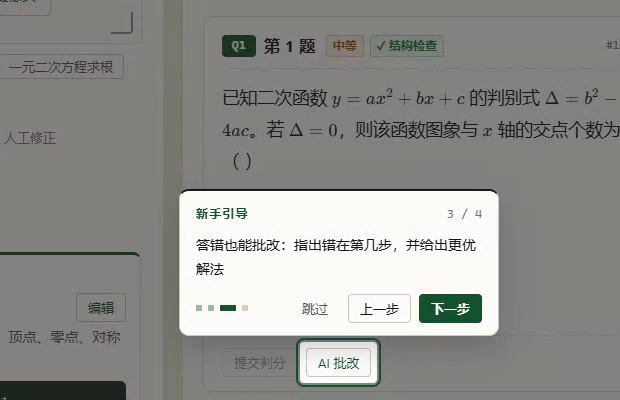
\includegraphics[width=0.58\textwidth,height=5.0cm,keepaspectratio]{img/c01.png}
\caption{四步新手引导中的批改版块。遮罩保留目标区域可见，说明分数、出错步骤和更优解法的入口。}
\label{fig:ui-tour}
\end{figure}

卡片区把模型结果保持为可编辑对象，而非只读摘要。标题、摘要、公式和正文均可修订，保存后当前列表就地更新，来源关系和创建时间不变。修改历史记录旧值与新值，刷新后仍可查看。这个入口位于识别和命题之间，使用户能够在错误进入练习前进行处理。

\begin{figure}[H]
\centering
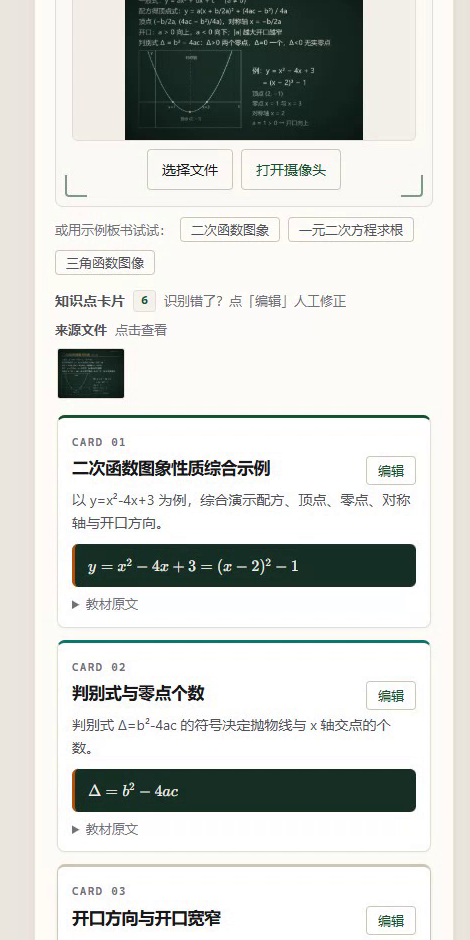
\includegraphics[height=7.7cm,keepaspectratio]{img/02-cards.png}
\caption{识别来源与知识卡片局部。卡片按字段展示，公式由 KaTeX 渲染，编辑入口用于人工修正与历史查看。}
\label{fig:ui-cards}
\end{figure}

\clearpage
\subsection{逐条出题、验算级别与分步批改}

出题结果按题逐条进入练习卷。卡片上的徽章区分“已验算”和“结构检查”，顶部汇总分别统计不同级别。题目进入列表不代表检查已经结束，质检事件继续更新状态。图中所示批次包含符号验算与结构检查两类结果，说明系统没有用同一“通过”标签掩盖检查深度。

\begin{figure}[H]
\centering
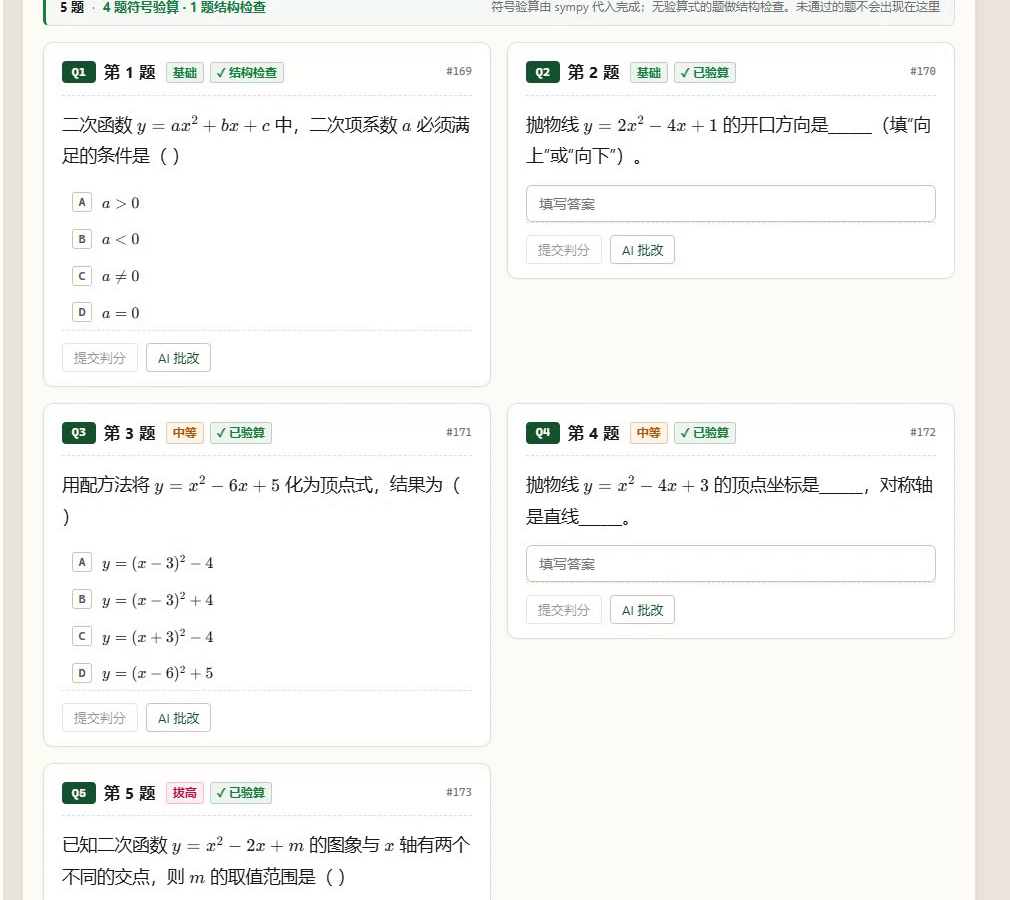
\includegraphics[width=0.69\textwidth,height=9.4cm,keepaspectratio]{img/c03.png}
\caption{命题结果与验收单局部。题目逐条出现，验算级别和批次汇总来自后端题目对象及结束事件。}
\label{fig:ui-questions}
\end{figure}

批改面板把分数与步骤诊断放在同一视图中。首个错误步骤被明确标出，后续区域给出原因和改进建议。分数环和步骤高亮由结构化结束事件驱动，连续评语由分片事件驱动，因此正文逐步出现时，步骤结论不会失去可核对性。mock 下只展示规则能够支持的诊断，不伪造学生方法归因。

\begin{figure}[H]
\centering
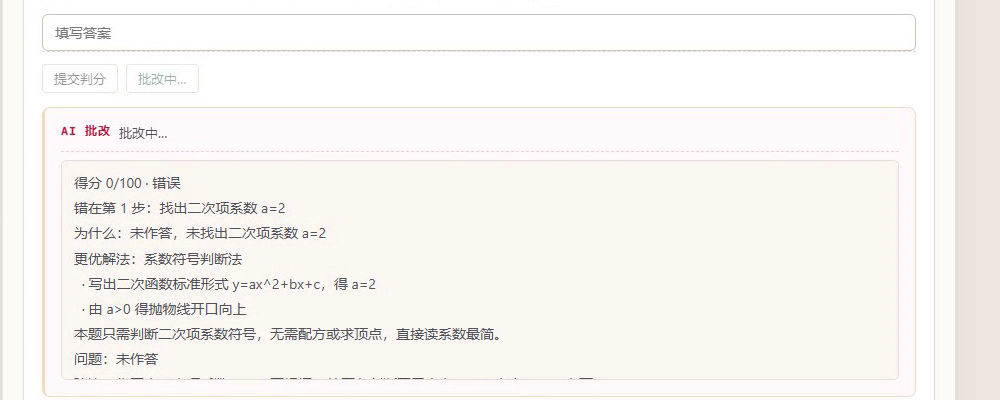
\includegraphics[width=0.96\textwidth,height=6.1cm,keepaspectratio]{img/c04.png}
\caption{AI 批改局部。示例定位到首个错误步骤，并给出错误原因、更优解法和后续建议。}
\label{fig:ui-review}
\end{figure}

\clearpage
\subsection{错题讲解函数图与知识谱系}

讲解图将抽象系数变成可拖动参数。当前二次函数模板固定观察范围，避免每次拖动都重新缩放坐标系。独立函数图入口允许输入受限表达式，解析失败时显示错误，不执行字符串代码。图像用于辅助理解，不代替步骤诊断，也不表示已经支持任意学科的可视化模板。

\begin{figure}[H]
\centering
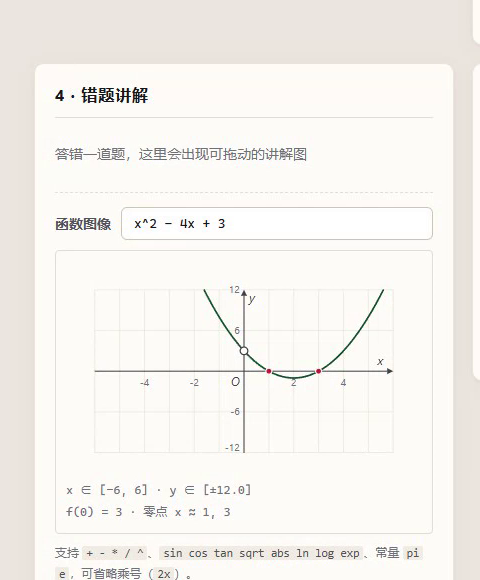
\includegraphics[height=9.5cm,keepaspectratio]{img/05-graph.png}
\caption{错题讲解与函数图局部。表达式、参数和图像保持同步，特殊点按可见范围绘制。}
\label{fig:ui-graph}
\end{figure}

知识谱系按共享标签建边，节点大小表示该卡片关联的出题量，颜色深浅表示被问次数，侧栏列出高频卡片。泛化程度过高的标签不用于建边，减少无意义的全连接。该图用于定位个人资料中的活跃主题，不作为学生掌握度评分。

\begin{figure}[H]
\centering
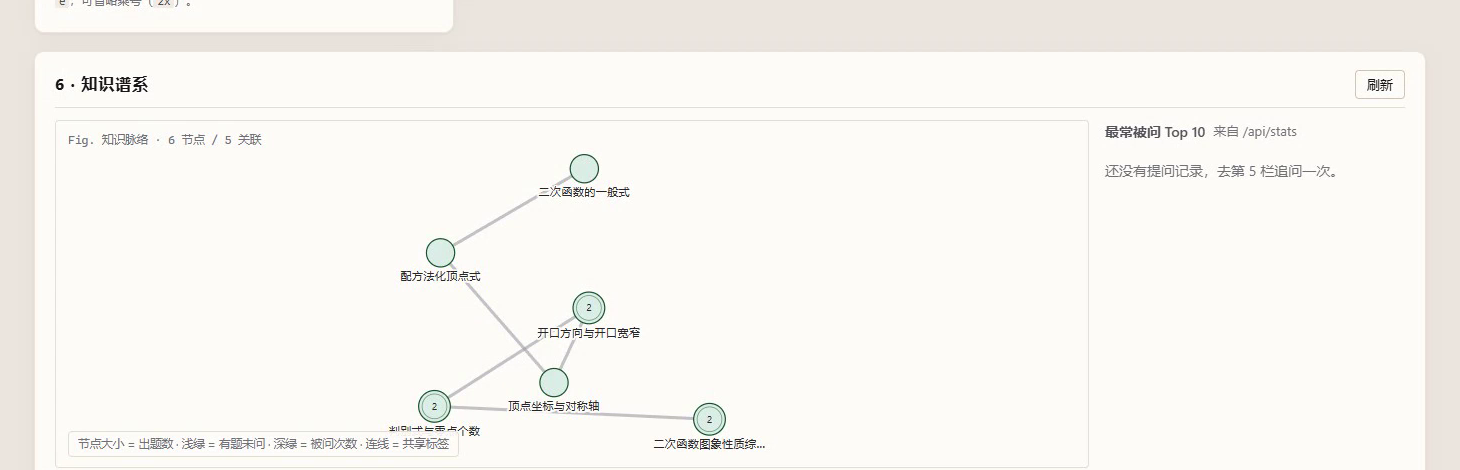
\includegraphics[width=0.97\textwidth,height=5.0cm,keepaspectratio]{img/c06.png}
\caption{知识谱系局部。节点、共享标签关系、原图入口与高频榜来自同一批本地卡片和计数。}
\label{fig:ui-lineage}
\end{figure}

\section{发表与获奖情况}

本作品此前未在期刊、会议、预印本平台或其他公开出版物发表，未登记为既有获奖成果，也未以当前完整作品形态参加其他比赛。本次为首次提交。与作品配套的技术文档、作品介绍、演示视频和界面截图均为本次赛事制作，没有将其他项目的材料改名后重复使用。

代码仓库应本次比赛要求公开，地址为 \textbf{\repo}。仓库为 Public，保留按功能模块和核心 AI 会话划分的提交记录。历史用于核对实现顺序和返工过程，不为参赛补造提交，不修改时间戳。仓库中的 README、技术文档、测试、评测结果和 AI 对话快照可与本文互相核对。

作品当前没有论文、专利、软件著作权或奖项可列示。本文不以“已申请”“在审”或“拟发表”等表述填补空白。若后续产生正式发表或获奖记录，应以可核验的公开链接、证书编号或官方页面另行更新，本节目前只陈述截至 2026 年 11 月 18 日的事实。

\begin{table}[H]
\centering\footnotesize
\caption{公开材料与核验入口}
\begin{tabularx}{\textwidth}{@{}L{3.0cm}Y L{3.5cm}@{}}
\toprule
\textbf{材料} & \textbf{位置} & \textbf{可核对内容} \\
\midrule
公开源码 & \repo & 业务实现、细粒度历史、许可与提交说明 \\
复现指南 & 仓库根目录 \file{README.md} & 环境要求、启动命令、配置、功能与边界 \\
技术文档 & \file{docs/技术文档.md} 及配套 PDF & 架构、意图控制、接口、测试、评测和局限 \\
AI 对话快照 & \file{docs/ai-logs/} & 关键提示词、人工采纳与否决、落地结果 \\
测试与评测 & \file{apps/server/tests/}、\file{apps/web/tests/}、\file{scripts/eval-results/} & 确定性断言、逐题或逐问句结果、统计口径 \\
\bottomrule
\end{tabularx}
\end{table}

\section{原创性与二次开发说明}

\subsection{业务设计与代码来源}

一纸成课为本赛事独立设计和实现的作品，不是对现有错题本、扫描、出题或在线课程项目的 fork，也没有在某个开源应用上更换名称和界面后提交。纸面到卡片的业务路径、七 Agent 分工、命题与质检反馈、三级验算语义、卡片修订历史、事件回放、函数图交互和知识谱系统计均围绕本作品需求开发。通用 Web 框架与符号计算库提供基础设施，不等同于复用已有同类作品。

开发过程中使用 AI 编码助手讨论方案、生成部分代码草稿、补充测试用例和开展独立评审。开发者负责确定 Must/Cut 范围、审查关键逻辑、选择是否采纳建议，并执行实际验收。架构上否决了超出当前需求的状态机框架、向量库和绘图库；安全上没有采用黑名单过滤建议，而是重新实现白名单解析；产品上没有把 mock 结果描述为真实识别。关键采纳与否决记录保存在 \file{docs/ai-logs/}，可以与提交历史及测试变化对照。

项目没有训练或微调自有基础模型。智谱、DeepSeek 以及配置中支持的其他 Provider 属于第三方模型与服务，运行时调用的模型能力不列为自研成果。自写 mock 样例用于复现和测试，三套教学内容不包含真实学生资料。BGE-M3 只在可选混合检索评测中作为现成嵌入模型使用，也不属于本作品训练的模型。

\subsection{第三方组件的边界}

FastAPI、React、sympy、PyMuPDF、PyInstaller、Electron、KaTeX、python-docx 等组件分别提供 Web 服务、界面、符号计算、文档处理、打包、桌面壳和公式渲染能力。它们按照各自许可证使用，依赖名称、用途和许可在附录 B 列出。仓库根目录的 \file{THIRD_PARTY_NOTICES.md} 与桌面资源中的许可证文本用于说明再分发义务。

源码采用 MIT 许可，但桌面二进制包含 PyMuPDF 等带有 AGPL 义务的组件。根许可证不能被描述为把所有组件都变成 MIT。公开源码、对应获取方式和 NOTICE 是当前交付采取的措施，若未来分发渠道要求整包采用另一种许可结构，需要更换组件或取得适当商业授权。该问题属于许可合规边界，不影响对业务代码原创来源的说明，但也不能被省略。

\begin{table}[H]
\centering\footnotesize
\caption{原创性核验对象与判断方式}
\begin{tabularx}{\textwidth}{@{}L{3.0cm}Y L{3.7cm}@{}}
\toprule
\textbf{对象} & \textbf{来源说明} & \textbf{核验方式} \\
\midrule
业务流程与数据结构 & 围绕纸面资料转学习动作独立设计，无同类项目 fork & 对照仓库初始设计、数据表和后续提交 \\
七 Agent 与反馈回路 & 按能力异构和独立否决需求实现，编排器为本项目代码 & 查看 \file{orchestrator.py}、Agent 文件和流水线测试 \\
前端交互与图形 & 单页六面板、事件看板、SVG 函数图和谱系为本项目实现 & 查看组件源码、前端纯函数测试与运行截图 \\
AI 辅助内容 & 草稿、候选用例和评审建议由 AI 参与，人工判断后落地 & 查看快照中的提示词、否决理由与对应提交 \\
教学样例与评测集 & 二次函数、一元二次方程、三角函数样例自写，评测为构造集 & 查看 fixtures、样例生成脚本和结果 JSON \\
基础库与模型 & 使用通用开源组件及第三方 API，不声称这些组件和模型自研 & 查看依赖锁文件、NOTICE、Provider 配置与附录 B \\
早期草稿与内部评审 & 未作为公开成果发表，不授权其他参赛作品重复使用 & 公开仓库只含本次交付所需材料，历史不补造 \\
\bottomrule
\end{tabularx}
\end{table}

原创性不等于每一行基础代码都由手工独立完成，也不等于没有使用通用库和 AI。这里的声明重点是：没有套用他人同类作品，业务设计与工程取舍可解释，第三方和 AI 的作用可核对，关键实现能够运行和测试。公开仓库的细粒度历史用于展示过程，不能单独作为原创性的唯一证明；源码、快照、测试和实际运行共同构成核验材料。

\clearpage
\appendix
\section{十分钟复现清单}

本清单以 Windows 源码模式为例，其他系统的差异只在虚拟环境激活命令。目标是在无 API Key、无 GPU 的条件下看到完整主路径。依赖下载时间受网络影响，表中的十分钟指常用网络和本机缓存条件下的操作预算，不把它作为所有机器的硬保证。追求最短现场启动时，优先使用已解压的 Windows 目录版。

\begin{longtable}{@{}L{0.8cm}L{1.3cm}L{7.1cm}L{5.5cm}@{}}
\caption{零密钥十分钟复现步骤}\label{tab:reproduce}\\
\toprule
\textbf{步骤} & \textbf{预算} & \textbf{命令或动作} & \textbf{通过标准} \\
\midrule
\endfirsthead
\toprule
\textbf{步骤} & \textbf{预算} & \textbf{命令或动作} & \textbf{通过标准} \\
\midrule
\endhead
1 & 0.5 min & \file{git clone https://github.com/Td12138/yizhi-chengke.git}，进入仓库 & 根目录可见 \file{apps/}、\file{docs/}、\file{README.md} \\
2 & 0.2 min & Windows 执行 \file{copy .env.example .env}；其他系统执行 \file{cp .env.example .env} & 根目录 \file{.env} 存在，两个 Provider 均为 mock \\
3 & 2--3 min & 在 \file{apps/server/} 创建 Python 3.11+ 虚拟环境并安装 \file{requirements.txt}；测试另装 \file{requirements-dev.txt} & 依赖安装无错误；不需要模型账号 \\
4 & 0.3 min & 在后端目录执行 \file{python -m uvicorn app.main:app --host 127.0.0.1 --port 8710} & 控制台显示监听 127.0.0.1:8710 \\
5 & 2--3 min & 另开终端，在 \file{apps/web/} 执行 \file{npm install} 和 \file{npm run dev} & Vite 显示 \url{http://127.0.0.1:5173} \\
6 & 0.2 min & 请求 \file{http://127.0.0.1:8710/api/health} & \env{ok=true}、两个 Provider 为 mock、\env{ready=true} \\
7 & 2 min & 打开页面，选择示例板书，生成 5 题，答错一题，再提交批改并追问 & 七 Agent 有状态；题目带级别；出现讲解、步骤诊断和引用 \\
8 & 可选 & 仓库根目录执行 \file{python -m pytest apps/server/tests -q} & 当前基线为 403 项通过；本机约 68 s \\
9 & 可选 & \file{apps/web/} 执行 \file{npm test} 与 \file{npm run build} & 18 项通过，类型检查与生产构建无错误 \\
\bottomrule
\end{longtable}

复现时建议先确认页面顶栏显示 \env{VLM: mock} 和 \env{LLM: mock}。缺省首轮 mock 命题会在第 4 题产生一次真实验算驳回，随后进入第二轮。若完全没有驳回，可能是样例或版本发生变化，应查看事件和测试，而不是手动伪造提示。若真实 Provider 显示未就绪，检查 Key、端点和模型名；系统不会把配置错误静默改成 mock。

演示前重置使用 \file{python apps/server/scripts/reset_demo.py}。该命令缺省保留原图，清理运行数据。需要删除归档图片时显式添加 \env{--purge-images}。桌面版使用包内重置脚本，执行前先退出程序。自动化测试自带临时数据目录，不需要为了跑测试而重置开发库。

\section{接口与配置表}

\subsection{HTTP 接口清单}

后端共有 17 个接口。异步任务接口立即返回 \env{run_id}，实际结果经 SSE 交付。查询接口同步返回，卡片修订是局部写操作。所有路径均以本机服务为预期部署环境，不包含鉴权字段。

\begin{longtable}{@{}L{1.2cm}L{4.7cm}L{4.7cm}L{4.5cm}@{}}
\caption{HTTP 接口、输入输出与用途}\label{tab:api}\\
\toprule
\textbf{方法} & \textbf{路径} & \textbf{请求到响应} & \textbf{说明} \\
\midrule
\endfirsthead
\toprule
\textbf{方法} & \textbf{路径} & \textbf{请求到响应} & \textbf{说明} \\
\midrule
\endhead
GET & \file{/api/health} & 六个就绪与 Provider 字段 & 配置与启动检查 \\
POST & \file{/api/ingest} & \env{multipart:file} $\to$ \env{run_id,kind} & 图片或文档识别、萃取与归档 \\
GET & \file{/api/events/{run_id}} & \env{text/event-stream} & 实时事件、迟到补发与保活 \\
GET & \file{/api/runs/{run_id}/events} & \env{run_id,events} & 已落库事件回放，无记录 404 \\
GET & \file{/api/cards} & \env{cards} & 最近 100 张卡片 \\
PATCH & \file{/api/cards/{id}} & 四个可选字段 $\to$ 完整卡片 & 白名单局部更新并留痕 \\
GET & \file{/api/cards/{id}/revisions} & \env{revisions} & 新到旧，最多 50 条 \\
GET & \file{/api/sources} & \env{sources} & 上传来源、卡片数与文件地址 \\
GET & \file{/api/sources/{id}} & 来源、原始块和卡片 & 不返回本机绝对路径 \\
GET & \file{/api/sources/{id}/image} & 文件二进制 & 按后缀返回 MIME，缺失 404 \\
GET & \file{/api/questions} & \env{questions} & 最近 50 道题 \\
POST & \file{/api/generate} & 卡片 ID、需求、题量 $\to$ \env{run_id} & 题量裁剪 1--12，空卡片取最近 3 张 \\
POST & \file{/api/grade} & 题号、作答 $\to$ \env{run_id} & 判分写 attempt，答错触发讲解 \\
POST & \file{/api/review} & 题号、作答 $\to$ \env{run_id} & 分步批改，结构结果随 done 返回 \\
POST & \file{/api/ask} & \env{query} $\to$ \env{run_id} & 检索作答并带出处 \\
GET & \file{/api/graph} & \env{nodes,edges,tags} & 共享标签边与卡片计数 \\
GET & \file{/api/stats} & \env{top_asked} & 高频卡片前 10 \\
\bottomrule
\end{longtable}

健康检查的六个字段为 \env{ok}、\env{vlm_provider}、\env{llm_provider}、\env{vlm_ready}、\env{llm_ready}、\env{ready}。真实 Provider 的就绪判断只检查 Key、地址和模型名是否齐全，不会为了健康检查额外调用付费接口。因此 \env{ready=true} 表示配置完整且服务已启动，不保证上游当时一定可用。

\subsection{主要配置项}

配置从仓库根 \file{.env} 或桌面版显式指定文件读取。已存在的系统环境变量优先，显式值优先于 Provider 预设。整数配置解析失败时退回默认并警告，带 BOM 的 UTF-8 文件和常见行尾注释可处理。密钥只应在本机配置，以下表格不包含任何真实值。

\begin{longtable}{@{}L{5.0cm}L{2.7cm}L{7.2cm}@{}}
\caption{主要环境变量、缺省值与回退行为}\label{tab:config}\\
\toprule
\textbf{变量} & \textbf{缺省值} & \textbf{作用与边界} \\
\midrule
\endfirsthead
\toprule
\textbf{变量} & \textbf{缺省值} & \textbf{作用与边界} \\
\midrule
\endhead
\env{VLM_PROVIDER} & mock & 视觉 Provider，可选 mock、qwen、glm；真实模式需 Key \\
\env{LLM_PROVIDER} & mock & 文本 Provider，可选 mock、deepseek、qwen、glm \\
\env{VLM_BASE_URL/API_KEY/MODEL} & 按预设或空 & 视觉端点、密钥与模型；显式值优先，密钥无预设 \\
\env{LLM_BASE_URL/API_KEY/MODEL} & 按预设或空 & 文本端点、密钥与模型；DeepSeek 只补文本预设 \\
\env{VERIFY_MAX_RETRY} & 2 & 首轮之后最多两次重试，总轮次最多 3 \\
\env{VERIFY_STRUCTURE_CHECK} & 1 & 无账单时做结构检查；设 0 恢复直接放行并标 unchecked \\
\env{VERIFY_DEGRADE_FORMAT} & 1 & 有限格式错误转结构检查；安全类拒绝不受影响 \\
\env{VERIFY_FALLBACK_ON_EXHAUST} & 1 & 重试耗尽且无通过项时，结构合格题可标级交付；设 0 严格拒绝 \\
\env{JUDGE_SYMPY_EQUIV} & 1 & 字符串与数值失败后追加符号等价；设 0 恢复旧规则 \\
\env{EVENT_PERSIST} & 1 & 事件落库；设 0 只保留内存事件 \\
\env{EVENT_PERSIST_RUNS} & 200 & 保留最近运行的数量，超过后裁剪旧事件 \\
\env{RETRIEVAL_MODE} & legacy & \env{legacy} 为 2-gram，\env{hybrid} 为向量与 RRF 可选增强 \\
\env{EMBED_BASE_URL/MODEL/API_KEY} & 空 & OpenAI 兼容嵌入端点；仅 hybrid 使用，故障回退 \\
\env{EMBED_TIMEOUT_SECONDS} & 10 & 嵌入请求超时 \\
\env{EMBED_BATCH_SIZE} & 16 & 单批嵌入文本数 \\
\env{EMBED_MAX_CHARS} & 1000 & 单卡送嵌入文本上限 \\
\env{HYBRID_CORPUS_LIMIT} & 500 & 向量路最多参与的卡片数 \\
\env{APP_HOST/APP_PORT} & 127.0.0.1 / 8710 & 后端监听；修改端口需同步开发代理 \\
\env{APP_DATA_DIR} & 仓库 data 或桌面用户目录 & 数据库与上传目录，测试会覆盖为临时路径 \\
\env{SERVE_WEB/WEB_DIST} & false / 前端 dist & 是否由后端托管已构建前端 \\
\env{WEB_CSP} & 1 & 托管前端时添加 CSP；设 0 仅供排障 \\
\env{YIZHI_ENV_FILE} & 空 & 桌面单文件版指向可执行文件旁配置 \\
\bottomrule
\end{longtable}

题量最小值、默认值和最大值分别为 1、5、12。图片与文档上限分别为 12 MB 和 20 MB，PDF 最多渲染前 3 页，单份文本最多 2 万字。检索固定返回前三条，向量余弦下限为 0.35，RRF 常数为 60。事件单 run 内存上限 500 条，保活间隔 15 秒。上述常量用于限制上下文、存储与资源消耗，不应被理解为已经经过大规模压测的最佳参数。

\section{测试矩阵}

本矩阵抽取主路径和高风险边界，便于评审不阅读全部测试源码也能复核覆盖意图。实际参数化用例多于表内行数，403 是 pytest 展开后的当前总数。命令与样本均使用自写数据，不包含真实密钥或个人信息。

\begin{longtable}{@{}L{1.3cm}L{3.4cm}L{5.5cm}L{5.0cm}@{}}
\caption{核心功能与异常路径测试矩阵}\label{tab:test-matrix}\\
\toprule
\textbf{编号} & \textbf{对象} & \textbf{输入或操作} & \textbf{期望结果与层级} \\
\midrule
\endfirsthead
\toprule
\textbf{编号} & \textbf{对象} & \textbf{输入或操作} & \textbf{期望结果与层级} \\
\midrule
\endhead
T01 & 上传后缀 & 不支持扩展名；超限图片或文档 & 400 或 413，不留下不完整文件；接口测试 \\
T02 & 正常图片 & PNG/JPG 等允许格式，12 MB 内 & 返回 \env{run_id} 与 image 类型；接口与 E2E \\
T03 & PDF 文本层 & 正常文本与少量空白尾页 & 文本层直读，不调用视觉模型；文档测试 \\
T04 & PDF 乱码 & 文本层不可读，真实 VLM 分支 & 前 3 页按 180 DPI 渲染后识别；MockTransport \\
T05 & 损坏文档 & 加密、零字节 PDF，损坏 DOCX & 即使 mock 也返回可读错误，不生成假卡片；单元测试 \\
T06 & DOCX/TXT/MD & 段落、表格、标题、不同编码 & 保持文档顺序与块类型；文档测试 \\
T07 & 原图归档 & 中文标题、非法字符、重名、无标题 & 清理名称、追加序号，无标题保留随机名；存储测试 \\
T08 & 卡片局部更新 & 改一个字段、提交同值、空 PATCH & 只改提交字段；同值不留历史；空修改幂等；接口测试 \\
T09 & 修订权限与历史 & 改来源字段、查不存在卡片、连续多次修改 & 来源字段不生效；404；历史新到旧且只记真实变化 \\
T10 & 命题数量 & 请求 0、5、20 或模型多返回 & 请求裁剪到 1--12，多返回部分截断；接口与单元测试 \\
T11 & 首轮驳回 & mock 第 1 轮第 4 题期望值为正 & 实际值 -1，驳回并进入第 2 轮；流水线测试 \\
T12 & 第二轮交付 & mock 第 2 轮全部账单自洽 & 命题共两次，五题交付，无运行错误；流水线测试 \\
T13 & 空结果与单题异常 & 模型返回空列表或某题字段类型损坏 & 不崩溃、不无限循环；异常限制在单题或明确运行错误 \\
T14 & 三级验算 & 有 verify、无 verify、关闭结构检查 & 分别得到 symbolic、structural、unchecked，界面与入库一致 \\
T15 & 结构检查 & 空题干、空答案、未知题型、坏选项、合法短题干 & 坏结构驳回，“解方程”等合法短题干不误伤 \\
T16 & 数值容差与期望 & 浮点误差、期望偏移、非数值或溢出期望 & 容差内通过，不自洽驳回，类型异常不拖垮整批 \\
T17 & 数学注入 & 动态导入、文件写入、eval/exec、属性链 & 全部拒绝，独立工作目录零新增文件；安全测试 \\
T18 & 代入与幂结构 & 表达式代入、布尔、容器、指数塔、嵌套幂 & 非数值拒绝；危险结构在求值前快速拒绝 \\
T19 & 正常数学兼容 & 多项式、sqrt、三角、log、pi、小指数 & 保持正确计算结果，防止白名单过严；单元测试 \\
T20 & 判分等价 & 方程交换、展开与因式、分数与小数、上标 & 等价答案判对；快速规则失败后走符号路径 \\
T21 & 判分反例 & \env{x=2} 对 \env{y=2}，\env{x/2=2} 对 2 & 均判错，不采用等号右端字面短路；单元测试 \\
T22 & 判分资源限制 & 高次幂、垃圾表达式、非法 LaTeX & 快速退回旧规则，不阻塞事件循环，不放宽结果 \\
T23 & 批改结构 & 完整、部分和错误作答；模型缺字段或错类型 & 分数、结论、步骤、首个错误完整且类型收敛 \\
T24 & 方法归因 & 字符串 false、空方法、另一种解法 & 布尔正确归一；空方法不输出；mock 不伪造归因 \\
T25 & 评语分片与回退 & 短尾片、中流异常、模型坏 JSON & 拼接不丢字不重叠；无“半句加全文”；事件标回退 \\
T26 & 检索基线 & “为什么这里要配方”与无关天气问题 & 前者命中正确卡片，后者返回空，不硬凑出处 \\
T27 & RRF 与缓存 & 两路排名、换模型、维度或有限数异常 & 共识卡片优先；换模型重嵌；坏向量拒绝 \\
T28 & 检索故障 & 无端点、超时、缓存数据库异常 & 自动回退 legacy，追问继续，事件注明路径 \\
T29 & 事件生命周期 & 迟到订阅、异常、容量超限、结束关闭 & 补发历史；终止事件保留；所有路径最终关闭 \\
T30 & 事件落库回放 & 写库失败、重启、旧 run 裁剪、未知 run & 实时流不受写库影响；重启可回放；未知返回 404 \\
T31 & 讲解参数 & 正常参数、NaN、字符串、反向区间 & 合法参数作图；非法参数只保留文字讲解 \\
T32 & 谱系与计数 & 泛化标签、无有效边、同批重复卡片、计数失败 & 过滤泛化边；同源链兜底；每卡只计一次；主任务继续 \\
T33 & 配置兼容 & BOM、行尾注释、坏整数、未知 Provider、显式覆盖 & 可解析或回默认；未知 Provider 不就绪；显式值优先 \\
T34 & 前端纯函数 & 上传闸门、题数、流式字段、批改清洗、回放合成 & 18 项通过，无浏览器和外部服务依赖 \\
T35 & 七条 E2E & 上传、出题、讲解、追问、批改、修订、回放 & 源码与打包版各 7/7；端口被占退出 2，不污染开发库 \\
\bottomrule
\end{longtable}

矩阵没有覆盖的项目同样需要记录：没有组件级视觉回归，没有多用户权限测试，没有高并发和长期稳定性测试，没有真实学生样本学习效果实验，没有所有 Provider 的真实联调。新增能力时应先在本矩阵加入可判定行，再实现功能。模型生成的候选用例必须经过人工复核，尤其要同时给出正例和反例。

\section{第三方依赖与许可}

下表列主要直接依赖和交付组件。传递依赖的完整许可文本以仓库和发布包中的 \file{THIRD_PARTY_NOTICES.md}、许可证文件及包管理锁文件为准。模型服务不是随源码再分发的软件组件，但其使用受各自服务条款约束。

\begin{longtable}{@{}L{3.5cm}L{3.0cm}L{4.2cm}L{4.0cm}@{}}
\caption{主要第三方组件、许可与用途}\label{tab:dependencies}\\
\toprule
\textbf{组件} & \textbf{许可} & \textbf{用途} & \textbf{交付边界} \\
\midrule
\endfirsthead
\toprule
\textbf{组件} & \textbf{许可} & \textbf{用途} & \textbf{交付边界} \\
\midrule
\endhead
FastAPI & MIT & HTTP 接口、参数校验与 ASGI 应用 & 后端直接依赖 \\
Uvicorn & BSD-3-Clause & ASGI 服务运行 & 单 worker 为当前运行方式 \\
python-multipart & Apache-2.0 & multipart 上传解析 & 上传接口直接依赖 \\
httpx & BSD-3-Clause & OpenAI 兼容模型与嵌入请求 & 支持 MockTransport 测试 \\
sympy & BSD-3-Clause & 受限表达式、代入验算与等价判分 & 不直接接受裸 \env{sympify} 输入 \\
pypdf & BSD-3-Clause & PDF 辅助处理与验证 & 后端直接依赖 \\
PyMuPDF & AGPL-3.0 或商业许可 & PDF 文本提取与页面渲染 & 桌面二进制包含，需保留对应义务 \\
python-docx & MIT & DOCX 段落与表格读取 & 后端直接依赖 \\
React & MIT & 单页界面与组件状态 & 前端运行时依赖 \\
TypeScript & Apache-2.0 & 类型检查与源码开发 & 构建工具，不是后端运行时 \\
Vite & MIT & 前端开发服务器与生产构建 & dist 不直接入库 \\
KaTeX & MIT & 题干与卡片公式渲染 & 错误时退回原文显示 \\
Electron & MIT & Windows 桌面壳、进程与配置定位 & 桌面分发组件 \\
PyInstaller & GPL-2.0+ 与打包例外 & 后端及 Python 运行时收集 & 按自身例外与 NOTICE 交付 \\
Playwright & Apache-2.0 & Chromium 端到端冒烟 & 开发与测试依赖，不是业务运行时 \\
SQLite & Public Domain & 本地结构化存储与 WAL & 随 Python 或运行环境使用 \\
Python & PSF License & 后端运行时 & 桌面包内置运行时并附许可 \\
Node.js & MIT & 前端构建与测试运行 & Web 开发环境需要，桌面用户无需另装 \\
\bottomrule
\end{longtable}

源码 MIT 许可只覆盖本项目可授权部分，不能覆盖第三方组件自身条款。特别是 PyMuPDF 的 AGPL 或商业许可选择需要在二进制分发时持续处理。发布包必须保留第三方 NOTICE、许可文本和对应源码获取说明。若后续更换 PDF 组件，应同步更新依赖锁、NOTICE、打包内容和本表，而不是只删除一行依赖。

\section{术语表}

\begin{longtable}{@{}L{3.4cm}L{11.5cm}@{}}
\caption{本文术语与项目内含义}\label{tab:glossary}\\
\toprule
\textbf{术语} & \textbf{定义} \\
\midrule
\endfirsthead
\toprule
\textbf{术语} & \textbf{定义} \\
\midrule
\endhead
Agent & 具有单一职责的异步处理单元。本文七个 Agent 不直接互相调用，由编排器传递状态 \\
Provider & 视觉或语言模型的可替换提供方。mock 与真实 API 实现同一调用边界 \\
mock & 内置自写样例 Provider。经过真实编排和规则，但视觉部分不读取图片语义 \\
Run / run\_id & 一次用户动作对应的运行及唯一编号，用于订阅、事件落库、恢复和排障 \\
RunContext & 单次运行的数据上下文，卡片、题目、作答和中间结果经它在 Agent 间传递 \\
SSE & Server-Sent Events。服务端向浏览器单向推送事件的 HTTP 流式协议 \\
delta & 增量事件，可携带逐题、逐卡或评语文本分片，不等同于最终结果 \\
rejected & 质检业务驳回状态，表示题目未通过当前检查，不表示系统异常 \\
verify 账单 & 命题模型提交的表达式、数值代入与期望值，用于本地独立核算 \\
symbolic & 符号验算级别，表示受限表达式已在给定代入下完成数值核算 \\
structural & 结构检查级别，只表示题干、答案、题型与选项形状符合要求 \\
unchecked & 未验算级别，保留关闭结构检查后的兼容行为，不形成内容质量证明 \\
safe\_math & 项目的受限数学解析入口，包含字符、标识符、代入值和幂结构白名单 \\
RRF & Reciprocal Rank Fusion，倒数排名融合。按两路检索名次合成分数，不直接混合异质量纲原始分 \\
2-gram & 中文相邻双字切片。项目用它避免依赖空白分词，并配合字段权重和分数下限 \\
BGE-M3 & 可选混合检索评测使用的现成嵌入模型，不是本作品训练的模型 \\
card\_revision & 卡片字段修订记录，保存旧值、新值和时间，与卡片更新在同一事务写入 \\
agent\_event & 落库运行事件，支持内存运行回收或服务重启后的结局恢复 \\
json-fallback & 批改模型或 JSON 路径不可用时回退本地规则的事件标记 \\
CSP & Content Security Policy。桌面壳和后端静态托管用于限制页面资源加载策略 \\
KaTeX & 前端公式渲染组件。公式语法失败时页面保留原文，不阻断整个界面 \\
WAL & SQLite 的预写日志模式，改善读写并发，但不等于支持任意规模服务 \\
结构降级 & 在限定条件下从符号验算退回结构检查，必须修改级别、记录原因并发出提示 \\
top-3 命中率 & 正确卡片是否出现在检索结果前三名的样本比例，不是答案文本准确率 \\
\bottomrule
\end{longtable}

\vspace{0.8em}
\begin{keybox}[文档结束与复核入口]
作品源码、复现命令、测试和公开材料统一从 \repo 获取。本文数字按 v0.1.6 现状整理。若代码后续变化，应同时更新版本、测试结果、配置表、接口表和边界说明，避免只修改功能清单。
\end{keybox}


\end{document}
